%==========================================================================================
%
%								Uniwersytet Zielonogórski
%
%						SZABLON PRACY DYPLOMOWEJ W PAKIECIE LaTeX
%							wykonany podczas zajęć seminaryjnych
%				pod przewodnictwem prof. dr hab. inż Dariusza Ucińskiego
%
%							 Damian Kowalów, Mariusz Buciakowski
%
% 				       Wydział Informatyki, Elektrotechniki i Automatyki
%						Instytut Sterowania i~Systemów Informatycznych
%
%							 Zielona Góra, kwiecień 2013
%			   (ostatnia modyfikacja: 15.11.2019 przez Paweł Jamroziak)
%==========================================================================================
%\documentclass[a4paper,12pt]{book}
\documentclass[a4paper,12pt,openany]{book}
% ------------------------------------------------------------------------
% pakiet do wzorów ams
% ------------------------------------------------------------------------
\usepackage{amsmath}
\usepackage{amssymb}

% ------------------------------------------------------------------------
% język polski
% ------------------------------------------------------------------------
\usepackage[polish]{babel}
\usepackage{polski}
\usepackage[utf8]{inputenc}
\usepackage[T1]{fontenc}

% ------------------------------------------------------------------------
% obsługa pdf
% ------------------------------------------------------------------------
\usepackage[pdftex,usenames,dvipsnames]{color}	%obsługa kolorów

% ------------------------------------------------------------------------
% wstawienie danych o autorze i pracy 
% ------------------------------------------------------------------------
\usepackage[pdftex,
                hidelinks=true,
				pagebackref=false,						% referencje w spisie literatury do strony na, której została użyta
				draft=false,								% draft
				pdfpagelabels=false,						%
				pdfstartview=FitV,						% lub FitH
				pdfstartpage=1,							% 
				bookmarks=true,							% zakładki w pliku pdf
				pdfauthor={Kacper Wojciechowski},						% należy wpisać autora pracy
				pdftitle={Praca inżynierska},			% 
				pdfsubject={Metody realizacji interfejsu sieciowego w modułach IoT},				% tytuł
				pdfkeywords={interfejs sieciowy, mikrokontroler, system wbudowany, iot},			% słowa kluczowe
				unicode=true]{hyperref}   


% ------------------------------------------------------------------------
%	style
% ------------------------------------------------------------------------
\usepackage{extsizes}							%więcej rozmiarów czcionek
\usepackage[a4paper,left=3.5cm,right=2.5cm,top=2.5cm,bottom=2.5cm]{geometry}
\usepackage{tocloft}								% format spisu treści
\usepackage{array}								% lepiej wyglądające tabelki
\usepackage[format=hang,
				labelsep=period,
				labelfont={bf,small},
				textfont=small]{caption}		% formatuje podpisy pod rysunkami i tabelami
\usepackage{floatflt}							% ładniejsze opisywanie obrazków tekstem
\usepackage{subfig}								% możliwość wstawiania figur w kolumnach
\usepackage{graphicx}							% do obsługi grafiki
\usepackage{here}									% wymuszanie położenia figury w danym miejscu
\usepackage{url}									% adresy internetowe
\usepackage{enumerate}							% modyfikowanie list wyliczeniowych np \begin{enumerate}[(a)]...
\usepackage{multirow}							% do tabel 
% ------------------------------------------------------------------------
% listingi
% ------------------------------------------------------------------------
\usepackage{listings}							% do wstawiania listingow programów




\usepackage{slantsc} % Pochyłe kapitaliki  np. \textsl{\textsc{Automatyka i robotyka}}

% ------------------------------------------------------------------------
% inne
% ------------------------------------------------------------------------
\usepackage{glossaries}

\usepackage{dashrule}
\usepackage{fancyhdr} 							% do stopki i nagłówka
\usepackage{calc}
\usepackage{packages/zmienne}					% zmienne dodatkowe używane min. w karcie pracy oświadczeniu i stronie tytułowej zebrane w jednym miejscu
\usepackage{packages/strona_tytulowa}
\usepackage{packages/oswiadczenie}
\usepackage{packages/karta_pracy}
\usepackage{packages/pusta_strona}
\usepackage{packages/wspolrealizacja}
\usepackage{longtable}							% do podziału tabel na wiele stron

\usepackage{listingsutf8}
\usepackage{longtable}

\lstset{
literate={ą}{{\k{a}}}1 {Ą}{{\k{A}}}1 {ć}{{\'c}}1 {Ć}{{\'{C}}}1 {ę}{{\k{e}}}1 {Ę}{{\k{E}}}1 {ł}{{\l{}}}1 {Ł}{{\L{}}}1 {ń}{{\'n}}1 {Ń}{{\'N}}1 {ó}{{\'o}}1 {Ó}{{\'O}}1 {ś}{{\'s}}1 {Ś}{{\'S}}1 {ż}{{\.z}}1 {Ż}{{\.Z}}1 {ź}{{\'z}}1 {Ź}{{\'Z}}1
}

% ------------------------------------------------------------------------
% kodowanie czcionek
% ------------------------------------------------------------------------
\usepackage[T1]{fontenc}
\usepackage{lmodern}\normalfont %to load T1lmr.fd 

% ------------------------------------------------------------------------
% do algorytmów
% ------------------------------------------------------------------------

\usepackage{algorithm}
\usepackage{algorithmic}
\floatname{algorithm}{Algorytm}

% ------------------------------------------------------------------------
% do nomenklatury
% ------------------------------------------------------------------------

\usepackage[section]{placeins}
\usepackage{nomencl}
\makenomenclature
\usepackage{makeidx}
\makeindex
\renewcommand{\nomname}{Spis ważniejszych symboli}
% na końcu pliku z nomenklaturą należy umieścić polecenie
% \printnomenclature
% plik należy dodać poleceniem \input
%% przykład treści pliku
%% \nomenclature{$\oplus$}{Dylatacja zbioru}
%% \printnomenclature

% ------------------------------------------------------------------------
% do bibliografii
% ------------------------------------------------------------------------
\usepackage[backend=bibtex, style=numeric, sorting=none]{biblatex}
%\addbibresource{Bibliografia/bibliografia.bib}
%\bibliographystyle{unsrt}

% ------------------------------------------------------------------------
%   Kropki po numerach sekcji, podsekcji, itd.
%   Np. 1.2. Tytuł podrozdziału
% ------------------------------------------------------------------------
\makeatletter
    \def\numberline#1{\hb@xt@\@tempdima{#1.\hfil}}                      %kropki w spisie treści
    \renewcommand*\@seccntformat[1]{\csname the#1\endcsname.\enspace}   %kropki w treści dokumentu
\makeatother

\makeatother
% ------------------------------------------------------------------------
% Definicje
% ------------------------------------------------------------------------
\def\nonumsection#1{%
    \section*{#1}%
    \addcontentsline{toc}{section}{#1}%
    }
\def\nonumsubsection#1{%
    \subsection*{#1}%
    \addcontentsline{toc}{subsection}{#1}%
    }
\reversemarginpar %umieszcza notki po lewej stronie, czyli tam gdzie jest więcej miejsca
\def\notka#1{%
    \marginpar{\footnotesize{#1}}%
    }
%\def\mathcal#1{%
%    \mathscr{#1}%
%    }

\newcommand{\myemptypage}{ \newpage  \thispagestyle{empty}~\newpage}
\usepackage{makecell}

%-------------------------------------------------------------------------
% listingi
%-------------------------------------------------------------------------
\definecolor{commentColor}{rgb}{0,0.643,0}
\definecolor{keywordColor}{rgb}{0,0,0.835}
\lstdefinestyle{praca}{basicstyle=\footnotesize\ttfamily,
                        keywordstyle=\color{keywordColor},
                        commentstyle=\color{commentColor},
                        numbers=left,
                        stepnumber=1,
                        numberstyle=\scriptsize,
                        numbersep=10pt,
                        basewidth=0.5em,
                        extendedchars=true,
                        frame=tb}

\newcommand{\cppcode}[3]{\vspace{8pt}\lstinputlisting[caption=#2, style=praca, language=C++, label=#3, xleftmargin=.02\textwidth, xrightmargin=.02\textwidth]{#1}}

%-------------------------------------------------------------------------
% stopka i nagłówek
%-------------------------------------------------------------------------
\setlength{\headheight}{15pt}

\pagestyle{fancy}
\renewcommand{\chaptermark}[1]{\markboth{#1}{}}
\renewcommand{\sectionmark}[1]{\markright{#1}{}}

\fancyhf{}
\fancyhead[LE,RO]{\thepage}
\fancyhead[RE]{\textit{\nouppercase{\leftmark}}}
\fancyhead[LO]{\textit{\nouppercase{\rightmark}}}

\fancypagestyle{plain}{ %
\fancyhf{}
\renewcommand{\headrulewidth}{0pt}
\renewcommand{\footrulewidth}{0pt}}

% ------------------------------------------------------------------------
% Inne
% ------------------------------------------------------------------------
\frenchspacing
\setlength{\parskip}{3pt}           	%odstęp pomiędzy akapitami
%\linespread{1.49}                    	%odstęp pomiędzy liniami (interlinia)
\setcounter{tocdepth}{3}
\setcounter{secnumdepth}{3}


% ------------------------------------------------------------------------
% Polskie podpisy
% ------------------------------------------------------------------------
\renewcommand{\figurename}{Figure}
\renewcommand{\tablename}{Table}

% ------------------------------------------------------------------------
% Bibliografia
% ------------------------------------------------------------------------
%\bibliographystyle{unsrt}					% kolejność według użycia
%\bibliographystyle{plain}					% kolejność alfabetyczna
\bibliography{Bibliografia/bibliografia.bib}
  
  

%==========================================================================================
% Deklaracja fontow kapitalikowych z kodowaniem T1
%==========================================================================================
\DeclareFontShape{T1}{lmr}{bx}{sc} { <-> ssub * cmr/bx/sc }{}
\DeclareFontShape{T1}{lmr}{bx}{scit}{<-> ssub * cmr/bx/scsl}{}
%==========================================================================================
% Inne deklaracje
%==========================================================================================



%==========================================================================================
% Dane na temat pracy do wypełnienia
%==========================================================================================
\author{inż. Kacper Wojciechowski}
\kierunek{Informatyka}
\grupa{21 INF-ZSI-SD}		% np. 101AiRDz
\title{Analiza porównawcza bibliotek uczenia maszynowego języka C++ na potrzeby zastosowań w biostatystyce}
\tytulAngielski{Comparative analysis of machine learning libraries in C++ for applications in biostatistics}
\uczelnia{Uniwersytet Zielonogórski}
\wydzial{Wydział Informatyki, Elektrotechniki i Automatyki}
\praca{Praca dyplomowa} % pozostawić właściwe
\promotor{Prof. dr hab. inż. Dariusz Uciński}
\konsultant{} 	% nie usuwać w~przypadku braku lecz pozostawić puste czyli: \konsultant{}
%\konsultant{}
\miasto{Zielona Góra}
\miesiac{czerwiec}	% miesiąc złożenia pracy
\rok{2023}
\dzien{dd} 			% dzień podpisania oświadczenia (cyfrowo) np. 10
\mm{mm} 				% miesiąc podpisania oświadczenia (cyfrowo) np. 01 (styczeń)

%==========================================================================================
% Uwaga! polecenie \myemptypage dodaje pustą stronę do treści. Praca oddana do dziekanatu powinna być zbudowana zgodnie z szablonem znajdującym się na stronie WEIT (z jedną stroną pustą następującą po karcie pracy), jednak jeżeli student planuje wydruk dla siebie, zalecane jest zastąpienie poleceń \newpage poleceniem \myemptypage. Skutkuje to utworzeniem bardziej przejrzystego układu zgodnego z zaleceniami pisania książek, czyli rozpoczynanie nowych treści na prawej stronie.
%==========================================================================================


%==========================================================================================
% Dokument glowny
%==========================================================================================
\begin{document}
\pagenumbering{roman}
%=========================================================================================
% Strona tytułowa
%=========================================================================================
\thispagestyle{empty}
\stronatytulowa

\thispagestyle{empty}
\pustastrona
\newpage
%=========================================================================================
% Oświadczenie o~współrealizacji pracy - w~przypadku braku zakomentować lub usunąć sekcję
%========================================================================================
%\autorDwa{Imię i~nazwisko współautora}
%\wspolrealizacjaTrescJeden{wykaz czynności wykonanych przez tę osobę}
%\wspolrealizacjaTrescDwa{wykaz czynności wykonanych przez tę osobę}
%\wspolrealizacja
%\newpage

\thispagestyle{empty}
\newpage

%========================================================================================
% Streszczenie
%========================================================================================
\normalsize

\subsection*{Summary}

	This dissertation aims to analyze and compare machine learning libraries available for C++ for use in biostatistics. The following chapters describe:

    \begin{itemize}
    	\item [$\bullet$] general problems encountered in the process of implementing machine learning solutions;
    	\item [$\bullet$] characteristics of biostatistics datasets used for testing chosen libraries;
    	\item [$\bullet$] control results of the methods selected for libraries comparison purpose;
    	\item [$\bullet$] Shogun, Shark-ML and Dlib libraries with implementations of selected machine learning methods;
    	\item [$\bullet$] summary of featurs offered by each library in respect to each other.
    \end{itemize}

\vspace{1cm}
\noindent\textbf{Keywords:} machine learning, C++, library, neural network, deep machine learning, shallow machine learning.

\newpage
%\myemptypage

%========================================================================================
% Spis tresci, spis tabel i~rysunków
%========================================================================================
%spis tresci
	\tableofcontents
	\newpage
	%\myemptypage
%spis rysunków
 	\listoffigures
	\newpage
	%\myemptypage
%spis tabel
	\listoftables
	\newpage
	%\myemptypage

%========================================================================================
% Licznik Stron
%========================================================================================
\newcounter{licznikStron}
\setcounter{licznikStron}{\value{page}}
\setcounter{licznikStron}{1}
\pagenumbering{arabic}
\setcounter{page}{\value{licznikStron}}

%========================================================================================
% Tresc
%========================================================================================
\chapter{Wstęp}
\section{Wprowadzenie} % -------------------------------------------------------------------------

We współczesnym stanie techniki coraz częściej można spotkać się z urządzeniami i programami o inteligentnych funkcjach, takich jak predykcja zjawisk na podstawie zestawu danych, rozpoznawanie obrazu, analiza mowy, czy przetwarzanie języka naturalnego. Znajdują one zastosowanie w różnych dziedzinach codziennego życia, m.in. w medycynie. W zależności od potrzeb, techniki uczenia maszynowego można wykorzystać do zastosowań medycznych, jak np. rozpoznawanie komórek rakowych na skanach rezonansem magnetycznym, podejmowanie decyzji na podstawie zbioru objawów obecnych u pacjenta, lub przewidywanie norm związków naturalnie występujących w organiźmie ludzkim w zależności od okoliczności i wyników pomiarów. 

Jedną z istotnych dziedzin medycyny jest biostatystyka, polegająca na wykorzystaniu analizy statystycznej do wnioskowania na podstawie zbiorów danych, takich jak rezultaty przeprowadzonych badań (np. morfologicznych, poziomu poszczególnych hormonów we krwii, itp.), informacji o nawykach żywieniowych oraz stylu życia pacjenta. Szczególnie istotną formą systemów operujących w tej dziedzinie są systemy eksperckie, wykorzystujące techniki płytkiego i głębokiego uczenia maszynowego w celu wspierania diagnozy stawianej przez wykwalifikowanych lekarzy. 

U podstaw wyżej wymienionych zagadnień leży implementacja rozwiązań opartych o teorię uczenia maszynowego, oraz wszelkie związane z tym problemy. W związku z tym na przestrzeni lat powstało wiele gotowych narzędzi, takich jak biblioteki i \textit{frameworki}, mające na celu wsparcie programistów w szybkim i prawidłowym wprowadzaniu rozwiązań sztucznej inteligencji na różne platformy docelowe oraz w różnych językach, począwszy od języka C++, przez Python, po środowiska takie jak Matlab. 

Istotnym krokiem w przygotowywaniu oprogramowania wykorzystującego sztuczną inteligencję jest prawidłowy wybór wspomnianych wcześniej narzędzi dokonywany na etapie projektowania, tak, aby oferowały one możliwości adekwatne do wymagań funkcjonalnych. Niniejsza praca dokonuje analizy porównawczej bibliotek uczenia maszynowego dla języka C++ w kontekście zastosowań w dziedzinie biostatystyki, celem umożliwienia czytelnikowi trafnego wyboru odpowiedniego narzędzia do realizacji projektu badawczego.

\section{Cel i zakres pracy} % ----------------------------------------------------------------------

Celem pracy jest przeprowadzenie analizy i przygotwanie zestawienia bibliotek do uczenia maszynowego dla języka C++, obrazując przykłady bazujące na zestawie danych biostatystycznych.

Zakres pracy obejmował:

\begin{itemize}
    \item [$\bullet$] Przegląd dostępnych bibliotek języka C++;
    \item [$\bullet$] Inżynierię i kształtowanie danych;
    \item [$\bullet$] Płytkie i głębokie uczenie nadzorowane;
    \item [$\bullet$] Kwestie wydajnościowe w dopasowywaniu i wdrażaniu modeli;
    \item [$\bullet$] Badania praktyczne w oparciu o zestaw danych medycznych i biologicznych.
\end{itemize}

\section{Struktura pracy} % ----------------------------------------------------------------------

Pierwszy rozdział przedstawia ogólnym zagadnieniem dotykanym przez pracę, począwszy dziedziny problemu i jej zastosowań, do istoty tematu pracy. Dodatkowo omawiany jest cel i zakres realizacji pracy, oraz jej strukturą.

Kolejny rozdział wprowadza czytelnika do tematu uczenia maszynowego, oraz napotykanych w nim problemów dotyczących złożoności obliczeniowej oraz zużycia zasobów. Stanowią one podstawę do zaproponowania języka C++ jako technologi wspierającej ich rozwiązanie przy pomocy bibliotek. 

Tematem rozdziału trzeciego jest przygotowanie elementów testowych do wykorzystania w późniejszej analizie porównawczej. Składa się na nie wybranie i przygotowanie do zestawu danych biostatystycznych do procesu uczenia oraz wybrane wzorcowych rozwiązań. Czytelnik przeprowadzony jest przez normalizację danych i selekcję najlepiej dopasowanych regresorów, oraz zostaje zapoznany z przykładowymi wynikami rozwiązań wzorcowych.

Dalsza część pracy składa się z bloku omówienia i analizy wybranych bibliotek uczenia maszynowego pod kątem określonych kryteriów. Pierwszą z nich, opisaną w rozdziale czwartym, jest biblioteka TensorFlow autorstwa Google. W poszczególnych sekcjach poruszone zostały tematy takie jak możliwe sposoby wdrożenia utworzonych w niej modeli, wymagana forma danych, dostępne funkcjonalności związane z danymi oraz modelami, a także dostępność źródeł informacji na temat sposobu pracy z biblioteką.  
\chapter{A practical take at machine learning}
\section{Modern problems}

Machine learning is based on advanced algorithms and complex data structures, performing calculations on training and validation datasets provided by the user, aswell as data received during their regular operation.

Some of the most basic models are created via techniques such as linear and non-linear regression, logistics regression or linear discriminant analysis. They result in shallow machine learning models, which have relatively small computational complexity to evaluate results of a dataset in comparison to other models \cite{shallow}.

Few of the more soffisticated methods are for example decision trees, based on algorythmical tree logic \cite{tree}. Each of the tree layer corresponds to the best predictor available at a current state, causing branching to specific values or ranges of values. The result calculation is achieved via traversing the tree from the root to one of its ending leafs. 

The most advanced, yet at the same time most demanding in complexity and memory types of models are neural networks.

Do najbardziej zaawansowanych, aczkolwiek także najbardziej wymagających obliczeniowo i pamięciowo technik uczenia maszynowego należą techniki uczenia głębokiego wykorzystujące sieci neuronowe, jak np. głębokie sieci neuronowe (ang. \textit{Deep Neural Network, DNN}) i splotowe sieci neuronowe (ang. \textit{Convolutional Neural Network, CNN}). U podstaw tych metod leży struktura sieci neuronowej, składająca się z warstwy wejściowej, jednej lub więcej warstw ukrytych posiadających neurony, oraz jednej warstwy wyjściowej. Każdy węzeł z poprzedniej warstwy połączony jest z każdym węzłem w następnej warstwie, lecz neurony znajdujące się w tej samej warstwie są wzajemnie niezależne. Każde połączenie posiada przypisaną wagę użytą do przeliczenia wartości wchodzącej do danego neuronu z danego sąsiada z poprzedniej warstwy. Wewnątrz peceptronu obliczana jest suma iloczynów wyjść z poprzednich neuronów i wag odpowiadających połączeniom, a następnie dla uzyskanej sumy obliczana jest wartość funkcji aktywacyjnej, która stanowi wartość wyjściową neuronu \cite{mit_neural}. Przykładowa sieć wykorzystująca pojedynczy neuron w pojedynczej warstwie ukrytej przedstawiona została na rys. \ref{fig:nn}. 

\begin{figure}[!ht]
    \centering
    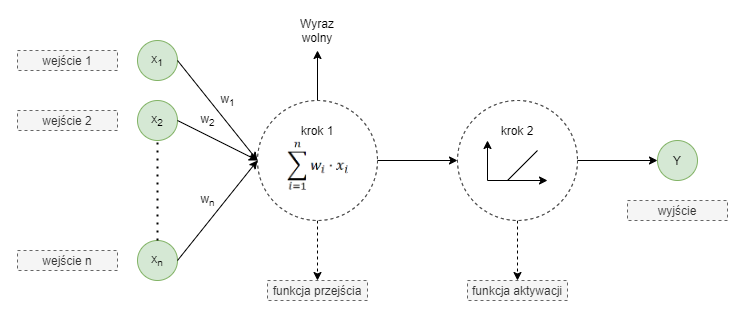
\includegraphics[width=150mm]{Rysunki/Rozdzial2/neuron.png}
    \caption{Schemat neuronu \dywiz{} Simplelearn.}
    \label{fig:nn}
\end{figure}

Bardziej rozbudowane metody wykorzystujące sieci neuronowe, jak np. CNN, wymagają dodatkowych kroków obliczeniowych związanych z wstępnym przetworzeniem danych wejściowych, aby były one przyswajalne dla wykorzystywanej sieci.

Analizując struktury danych wymagane przez poszczególne omówione powyżej rodzaje modeli, wyróżnić można następujące problemy napotykane podczas implementacji metod uczenia maszynowego \cite{constrained}:

\begin{itemize}
    \item [$\bullet$] Wymagania wydajnościowe -- są one ściśle powiązane ze złożonością obliczeniową wykorzystanych metod, wydajnością zastosowanego języka i wydajnością zastosowanej platformy sprzętowej. Docelowym efektem jest minimalizacja czasu wymaganego na uczenie modelu (chodź tutaj tolerowane są także długie czasy, szczególnie w przypadku dużych zestawów danch uczących) i czasu propagacji modelu (w przypadku czego minimalizacja czasu propagacji stanowi priorytet).
    
    \item [$\bullet$] Wymagania pamięciowe -- wynikają one z wykorzystywanych platform sprzętowych i ich ograniczeń pamięciowych. Przykładem powyższego dylematu jest zastosowanie modeli uczenia maszynowego na platformach mobilnych i platformach systemów wbudowanych, gdzie obecne rozmiary pamięci RAM i pamięci masowej (szczególnie w przypadku platform wbudowanych) potrafią być wyraźnie ograniczone w stosunku do systemów komputerowych.
\end{itemize}

W trakcie rozwoju technologii uczenia maszynowego, postawiono stanowcze kroki w kierunku rozwiązywania powyższych problemów, aby sprostać narastającym wymaganiom związanym z coraz to nowymi i bardziej skomplikowanymi zastosowaniami sztucznej inteligencji. Dokonywano tego poprzez m.in. optymalizację algorytmów, dobór platform sprzętowych o wysokim taktowaniu, możliwym zrównolegleniu operacji, oraz wykorzystaniu wysoko wydajnych języków programowania, w szczególności języków mających możliwość wykorzystania wsparcia ze strony operacji niskopoziomowych.

\section{Język C++ jako narzędzie do rozwiązania problemów uczenia maszynowego}

Dostępne są różne języki i środowiska wspierające uczenie maszynowe, począwszy od języków takich jak Python, C++, Java czy Matlab. Jednak spośród wymienionych kandydatów szczególnie istotnym wyborem jest język C++. 

C++ to język imperatywny charakteryzujący się silnym typowaniem, łączący programowanie niskopoziomowe dla konkretnych architektur z wysokopoziomowym programowaniem, w związku z czym oferuje programistom dużą kontrolę nad wykorzystaniem pamięci i możliwość optymalizacji w postaci m.in. dostosowywania wykorzystanych typów danych do wymagań funkcjonalnych tworzonej sieci, kontroli lokalizacji zmiennych (programista decyduje czy zmienna lub struktura znajdzie się na stosie czy stercie) oraz optymalizację czasów wywołań funkcji poprzez sugerowanie kompilatorowi utworzenia funkcji inline. W przeciwieństwie do języków skryptowych których kod jest interpretowany w trakcie wykonywania, takich jak Python i język środowiska Matlab, C++ jest językiem kompilowanym. Oznacza to, że program napisany w C++ przetwarzany jest z postaci tekstu do wykonawczego kodu binarnego dostosowanego do wybranej architektury procesora. Usuwa to całkowicie nadmiar złożoności obliczeniowej wykonywanego programu związanej z interpretacją poleceń i tłumaczeniem ich na język procesora danej platformy w trakcie wykonywania programu, gdyż jest to wykonywane tylko raz, na etapie kompilacji, dodatkowo pozwalając na zastosowanie przez kompilator mechanizmów optymalizacji dostępnych dla wybranej platformy \cite{cpp_char}. 

Część mechanizmów z języka C++, wywodzących się jeszcze z języka C, pozwala na wykorzystanie wstawek kodu źródłowego w języku Assembler dla wybranego procesora, co zwiększa wydajność programu kosztem przenośności kodu. Dodatkowo niektóre platformy oferują API modułów akceleracji sprzętowej (jak np. system Android udostępniający \textit{Neural Networks API, NNA} dla sieci neuronowych), co oferuje dodatkowe przyspieszenie czasu działania programu \cite{android_nna}.

\begin{figure}[!ht]
    \centering
    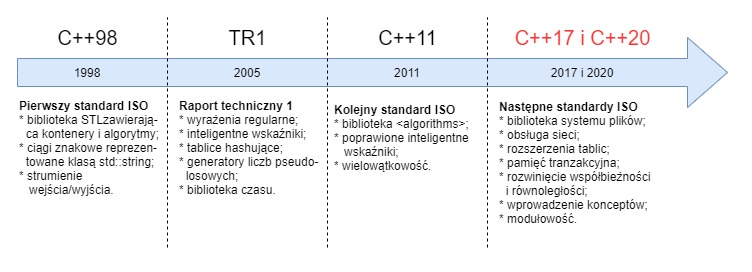
\includegraphics[width=150mm]{Rysunki/Rozdzial2/multithreading.jpg}
    \caption{Rozwój wielowątkowości w nowoczesnym C++ - Modernes C++.}
    \label{fig:cpp_history}
\end{figure}

Jedną z popularnych technik mających na celu znaczne zwiększenie wydajności modeli sztucznej inteligencji jest zrównoleglenie przetwarzania. Dostępność mechanizmów wielowątkowych dla procesorów (wprowadzonych w standardzie C++11 i dalej rozwijanych, jak przedstawiono na rys. \ref{fig:cpp_history}), oraz kompatybilność języka C++ z językiem CUDA \cite{cpp_cuda} pozwala wykonywać wiele obliczeń równolegle poprzez wykorzystanie wielu rdzeni lub oddelegowaniu części przetwarzania do karty (lub wielu kart) graficznej (gdzie liczba procesorów GPU znacząco przewyższa liczbę rdzeni CPU). Dodatkowym atutem wykorzystania języka C++ przy tworzeniu modelu sztucznej inteligencji jest łatwa integracja z programami dedykowanymi do wysokiej wydajności, napisanymi w tym języku.

Wymienione wyżej mechanizmy i cechy charakterystyczne języka umożliwiają programistom znaczną optymalizację przygotowywanych rozwiązań sztucznej inteligencji, co przekłada się na bardziej efektywne zużycie pamięci, zabezpieczenie przed przeładowaniem stosu procesora, oraz krótsze czasy propagacji utworzonych modeli.

\section{Cel powstania bibliotek}

Implementacja mechanizmów pozwalających na tworzenie rozwiązań sztucznej inteligencji, z racji na swoją złożoność, wymagania dotyczące kompetencji twórców oraz konieczność optymalizacji, jest czasochłonna i kosztowna. Tu z pomocą przychodzą biblioteki utworzone przez korporacje oraz społeczność programistów \textit{open source}. Stanowią one gotowe zbiory mechanizmów (najczęściej pisane w sposób obiektowy, a więc ubrane w klasy posiadające określone zestawy metod), które są na bieżąco optymalizowane przez grupy programistów wykorzystujące je w prywatnych projektach lub pracy zawodowej. Oferują one możliwość wykorzystania gotowych modeli utworzonych w innych technologiach, a czasem także bezpośrednie przygotowanie modelu na podstawie odpowiednio sformatowanego i odpowiednio przystosowanego zestawu danych.

Użycie gotowych bibliotek nie tylko redukuje koszty i przyspiesza tworzenie pożądanego rozwiązania sztucznej inteligencji, lecz także zapewnia większą niezawodność, gdyż elementy zawarte w bibliotece są implementowane, dokładnie testowane i poprawiane przez programistów o wysokich kompetencjach, jak m.in. w przypadku biblioteki TensorFlow posiadającej wsparcie od pracowników Google.

Większość bibliotek przeznaczonych do uczenia maszynowego, nawet wykorzystywanych w językach takich jak Python, napisana jest w języku C++, oferując API dostępne dla określonych języków docelowych. Niestety, nie wszystkie biblioteki napisane w ten sposób oferują dostęp do całego API w języku C++ dla wykorzystujących je programów zewnętrznych, lub bywa on utrudniony i skomplikowany, co sprawia że w powszechnej praktyce część bibliotek dedykowanych językowi C++ operuje na modelach przygotowanych w ramach innej, lub czasem nawet tej samej biblioteki, napisanych w innym języku. Częstym przypadkiem jest tutaj wykorzystanie właśnie języka Python do utworzenia grafu modelu lub modelu w formacie ONNX (ang. \textit{Open Neural Network Exchange}) \cite{cpp_onnx}. 

W ramach analizy porównawczej w niniejszej pracy, porównywane będą biblioteki oferujące zarówno tworzenie modeli w ramach języka C++, jak i wymagające wykorzystania modeli z innego źródła. 
\chapter{Inżynieria danych eksperymentalnych i testowe szablony modeli}
\section{Omówienie danych eksperymentalnych}

W celu zestawienia funkcjonalnego bibliotek uczenia maszynowego w języku C++ i przedstawienia przykładów konieczne było wybranie danych eksperymentalnych możliwych do wykorzystania jako porównawczy punkt odniesienia. W tym celu, dla pełnego przetestowania wybranych funkcjonalności przygotowano zestaw danych do problemu klasyfikacji binarnej oraz zadania regresji.

\subsection{Dane klasyfikacyjne}
	
	 Jako dane klasyfikacyjne wybrano bazę dotyczącą diagnostyki raka piersi ,,\textit{Wisconsin Diagnostic Breast Cancer}'' z listopada 1995 roku, w której zamieszczono wyniki obrazowania określone w sposób liczbowy. Autorami zestawu są Dr. Wiliam H. Wolberg, W. Nick Street oraz Olvi L. Mangasarian z Uniwersytetu Wisconsin \cite{wisconsin}. Baza ta jest dostępna do pobrania z repozytorium Uniwersytetu Californii \cite{Dua:2019}. Dane mają następującą strukturę:
	
	\begin{enumerate}
		\item [1)] ID - numer identyfikacyjny pacjentki;
		\item [2)] Diagnosis [\textit{Malignant - M} / \textit{Benign - B}] - charakter nowotworu, \textbf{zmienna odpowiedzi};
		\item [3)] Dane klasyfikujące:
			\begin{enumerate}
				\item [a)] \textit{Radius} - średnica guza;
				\item [b)] \textit{Texture} - tekstura guza;
				\item [c)] \textit{Perimeter} - obwód guza;
				\item [d)] \textit{Area} - pole guza;
				\item [e)] \textit{Smoothness} - gładkość, miara lokalnych różnic w promieniu guza;
				\item [f)] \textit{Compactness} - zwartość, wykorzystywana do oceny stadium guza;
				\item [g)] \textit{Concavity} - stopień wklęsłości miejsc guza;
				\item [h)] \textit{Concave points} - punkty wklęsłości guza;
				\item [i)] \textit{Symmetry} - symetria guza, pomagająca w ocenie charakteru przyrostu guza.
				\item [j)] \textit{Fractal dimention (,,coastline approximation'' - 1)} - wymiar fraktalny pozwalający na ilościowy opis złożoności komórek nerwowych, umożliwiający stwierdzenie nowotworzenia się zbioru komórek.
			\end{enumerate}
	\end{enumerate}
	
	Dla każdej ze zmiennych odpowiedzi została zebrana średnia wartość, odcyhelenie standardowe oraz średnia trzech największych pomiarów, gdzie każdy zestaw ustawiony jest sekwencyjnie (np. kolumna 3 - średni promień, kolumna 12 - odchylenie standardowe promienia, kolumna 22 - średnia trzech największych pomiarów promienia). Każda ze zmiennych ma charakter ciągły. Zredukowany zestaw danych, zawierający jedynie zmienne decyzyjne informujące o średnich wartościach znaleźć można jako dodatek do książki ,,\textit{Biostatistics Using JMP: A Practical Guide}'' autorstwa Trevora Bihla \cite{biostatisticsJMP}.
	
\subsection{Dane regresyjne}

	Do demonstracji problemu regresji wykorzystano zestaw danych ,,IronGlutathione'' dołączony do książki ,,Biostatistics Using JMP - A Practical Guide'' autorstwa Trevora Bihla \cite{biostatisticsJMP}, dotyczące badań nad związkiem między zawartością żelaza, a $\alpha$- i $\pi$-glutathonine-s-transferase w organiźmie człowieka. Obserwacje pochodzą z badań z 2012 roku. Zestaw posiada 90 obserwacji i składa się z 10 zmiennych:
	
	\begin{enumerate}
		\item \textit{Age} - wiek badanej osoby;
		\item \textit{Gender} - płeć osoby;
		\item \textit{Alpha GST (ng/L)} - zawartość transferazy glutatoninowej typu $\alpha$;
		\item \textit{pi GST (mg/L)} - zawartość transferazy glutatoninowej typi $\pi$;
		\item \textit{transferrin (mg/mL)} - zawartość transferyny;
		\item \textit{sTfR (mg/mL)} - zawartość rozpuszczalnego receptora transferyny;
		\item \textit{Iron (mg/dL)} - zawartość żelaza;
		\item \textit{TIBC (mg/dL)} - całkowita zdolność wiązania żelaza;
		\item \textit{\%ISAF (Iron / TIBC)} - współczynnik nasycenia transferyny;
		\item \textit{Ferritin (ng/dL)} - zawartość ferrytyny;
	\end{enumerate} 
	
	Z racji na większą swobode w wyborze zmiennej odpowiedzi w przypadku danych regresyjnych, zdecydowano się na wybór ostatniej zmiennej (\textit{Ferritin (ng/dL)}) jako przewidywaną zmienną odpowiedzi. 
	
\section{Charakterystyka i przetwarzenie danych}

	W celu przeprowadzenia procesu uczenia maszynowego, jednym z najistotniejszych kroków jakie należy podjąć jest wstępne zaznajomienie się z zestawem danych i jego analiza pod kątem rozkładu poszczególnych zmiennych oraz prawdopodobieństw. W tym celu wykorzystane zostało oprogramowanie JMP. 

	\subsection{Dane klasyfikacyjne}
	\subsubsection{Analiza rozkładu danych}
		
	Proces analizy rozkładu rozpoczęty został od przyjrzenia się zmiennej odpowiedzi (\textit{Diagnosis}). Rysunek \ref{fig:diagnosisdistribution} przedstawia uzyskany histogram, wraz z tabelą określającą ilość obserwacji danej klasy i współczynnik prawdopodobieństwa przynależności odpowiedzi do danej klasy. Zauważyć można, że dla użytego zestawu danych ilość zarejestrowano 357 obserwacji łagodnego raka piersi, a jego prawdopodobieństwo przynależności do klasy \textit{Benign} wynosi $\approx$ 62,7\%, natomiast do klasy \textit{Malignant} przynależało 212 obserwacji z prawodpodobieństwem $\approx$ 37,3\%.
		
	Podczas analizy histogramów zmiennych decyzyjnych, stwierdzono że znaczna ilość ma charakter prawostronnie skośny oraz występują dla nich obserwacje odstające, o czym informuje znajdujący się po prawej stronie histogramu wykres okienkowy (ang. \textit{box graph}), co przedstawiono na rysunku \ref{fig:variabledistribution}. Wyjątkiem okazała się zmienna \textit{Mean Largest Concave Points}), która mimo lekkiej skośności, okazała się nie posiadać obserwacji odstających. Na podstawie tych informacji stwierdzono, że aby przygotować dane w odpowiedni sposób do procesu uczenia należy przeprowadzić ich czyszczenie oraz normalizację rozkładu.
	
	\begin{figure}[!ht]
		\centering
		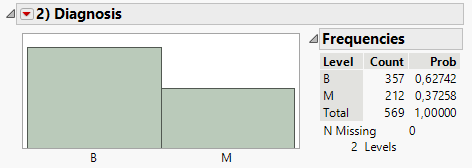
\includegraphics[width=0.6\linewidth]{Rysunki/Rozdzial2/diagnosis_distribution}
		\caption{Histogram rozkładu zmiennej odpowiedzi}
		\label{fig:diagnosisdistribution}
	\end{figure}
	
	\begin{figure}[!ht]
		\centering
		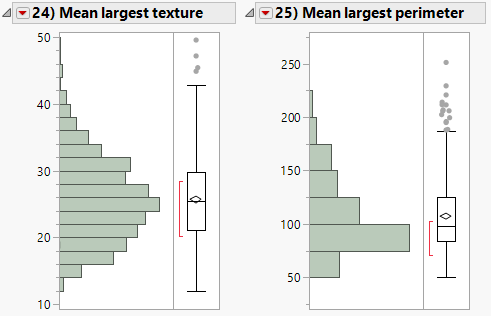
\includegraphics[width=0.6\linewidth]{Rysunki/Rozdzial2/variable_distribution}
		\caption{Przykłady histogramów zmiennych decyzyjnych}
		\label{fig:variabledistribution}
	\end{figure}
	
	
	\subsubsection{Czyszczenie i normalizacja rozkładu danych}
	
	Na pełny zestaw danych składa się 569 obserwacji. Podczas wstępnej analizy stwierdzono istnienie 13 brakujących wartości dla regresora \textit{Std err concave points}, dla których przyjęto wartość średnią z całej kolumny. Głównym problemem okazały się obserwacje odstające oraz skośności rozkładu. Do analizy obserwacji odstających wykorzystano wykresy okienkowe, gdzie oś Y reprezentowała zmienną odpowiedzi, natomiast oś X czyszczoną zmienną decyzyjną. Przykładowy wykres został przedstawiony na rysunku \ref{fig:boxgraph}. Ze względu na bardzo małą ilość obserwacji zdecydowano się rozpocząć proces przystosowywania danych do uczenia poprzez normalizację ich rozkładu, aby zminimalizować lub wyeliminować konieczność usunięcia danych odstających. 
	
	\begin{figure}[!ht]
		\centering
		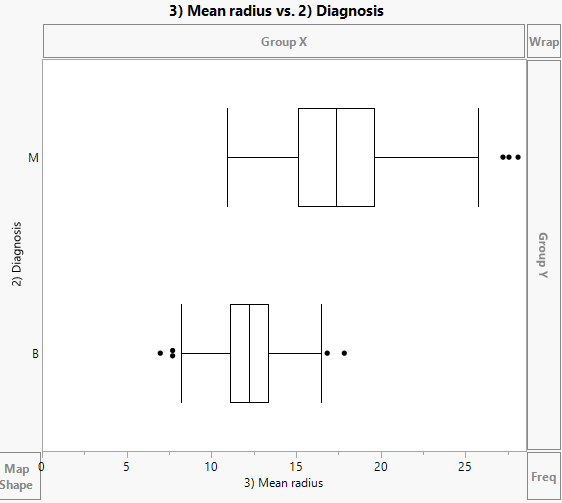
\includegraphics[width=0.7\linewidth]{Rysunki/Rozdzial2/box_graph}
		\caption{Przykład analizy obserwacji odstających dla poszczególnych klas zmiennej odpowiedzi}
		\label{fig:boxgraph}
	\end{figure}

	\newpage
	
	W pierwszym podejściu zdecydowano się na zastosowanie transformacji logarytmicznej dla wszystkich zmiennych decyzyjnych i porównanie charakterystyk uzyskanych rozkładów z oryginalnymi. Zmienna \textit{Mean largest concave points} okazała się posiadać rozkład bardzo zbliżony do standardowego, w związku z czym wyłączono ją z dalszej analizy normalizacji. Przykładowe wyniki przedstawiono na rysunku \ref{fig:log}. Transformacja ta okazała się skutecznym rozwiązaniem jedynie dla następujących zmiennych:
	
	\begin{enumerate}
		\item \textit{Mean radius};
		\item \textit{Mean texture};
		\item \textit{Mean perimeter},
		\item \textit{Mean area};
		\item \textit{Mean smoothness};
		\item \textit{Mean symmetry};
		\item \textit{Std err texture};
		\item \textit{Std err smoothness};
		\item \textit{Std err compactness};
		\item \textit{Std err concave points};
		\item \textit{Mean largest texture};
		\item \textit{Mean largest smoothness};
		\item \textit{Mean largest compactness}.
	\end{enumerate}

	\begin{figure}[!ht]
		\centering
		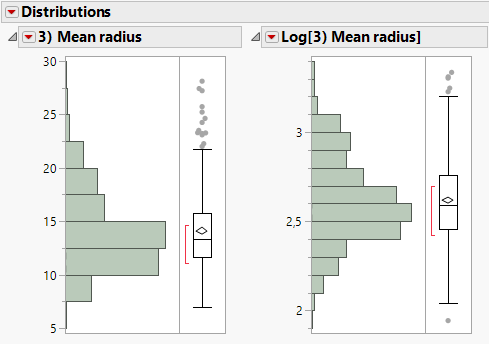
\includegraphics[width=0.7\linewidth]{Rysunki/Rozdzial3/log}
		\caption{Porównanie rozkładu danych przed i po transformacji logarytmicznej.}
		\label{fig:log}
	\end{figure}

	W drugim kroku podjęto próbę wykorzystania transformacji pierwiastkiem sześciennym dla pozostałych zmiennych decyzyjych, ze względu na jej skuteczność dla danych o rozkładzie prawoskośnym. Rysunek \ref{fig:cuberoot}. przedstawia porównanie rozkładu zmiennej \textit{Mean concavity} przed i po transfromacji pierwiastkiem sześciennym. Pomyślnie znormalizowano rozkład następujących zmiennych:
	
	\begin{enumerate}
		\item \textit{Mean compactness};
		\item \textit{Mean concavity};
		\item \textit{Mean concave points};
		\item \textit{Std err concavity};
		\item \textit{Mean largest radius};
		\item \textit{Mean largest perimeter};
		\item \textit{Mean largest concavity};
		\item \textit{Mean largest symmetry}.
	\end{enumerate} 

\begin{figure}[!ht]
	\centering
	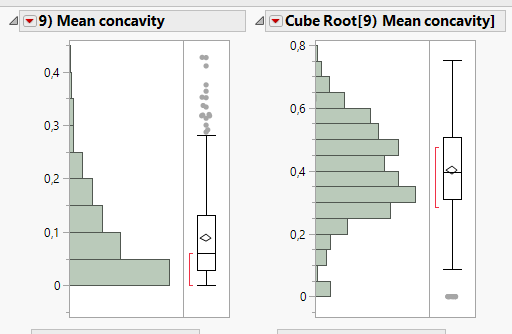
\includegraphics[width=0.7\linewidth]{Rysunki/Rozdzial3/cube_root}
	\caption{Porównanie rozkładów danych przed i po zastosowaniu transformacji pierwiastkiem sześciennym.}
	\label{fig:cuberoot}
\end{figure}

	Ostatecznym krokiem okazało się zastosownie odwrotnej transformacji Arrheniusa, Niestety część z uzyskanych zmodyfikowanych zmiennych decyzyjnych zachowała częściowy skośny rozkład, jednak inne przetestowane transformacje, jak m.in. pierwiastek kwadratowy, potęga kwadratowa, logarytm x+1, logarytm dziesiętny, funkcja potęgowa, funkcja wykładnicza, przyniosły rezultaty porównywalne lub gorsze od uzyskanego w wyniku w/w odwrotnej transformacji Arrheniusa. Rysunek \ref{fig:arrhenius} przedstawia porównanie uzyskanych rozkładów.
	
	\begin{figure}[!ht]
		\centering
		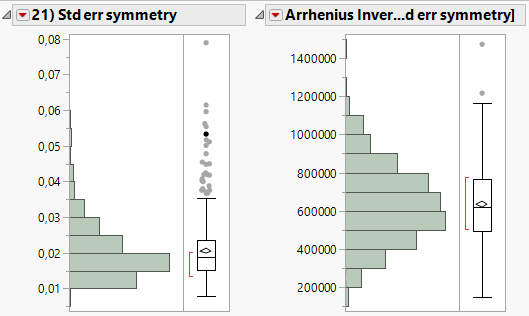
\includegraphics[width=0.7\linewidth]{Rysunki/Rozdzial3/arrhenius}
		\caption{Porównanie uzyskanych rozkładów danych przed i po odwrotnej transformacji Arrheniusa.}
		\label{fig:arrhenius}
	\end{figure}
	
	Ze względu na bardzo małą ilość obserwacji, zdecydowano się na zachowanie wszystkich obserwacji odstających, aby zapobiec utracie informacji i zmianie uzyskanych w procesie normalizacji rozkładów. W celu zachowania kompatybilności z bibliotekami omawianymi w niniejszej pracy, przekodowano zmienną odpowiedzi na wartości liczbowe.

	\subsection{Dane regresyjne}
	
	\subsubsection{Analiza rozkładu danych}
	
	Podobnie jak w przypadku danych klasyfikacyjnych, analizę rozpoczęto od zapoznania się z rozkładem wybranej zmiennej odpowiedzi. Zauważono że posiada ona rozkład skrajnie prawostronny, co przedstawiono na rysunku \ref{fig:ferritin}.
	
	\begin{figure}[!ht]
		\centering
		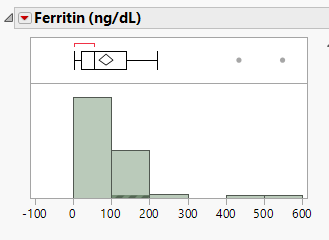
\includegraphics[width=0.5\linewidth]{Rozdzial3/ferritin}
		\caption{Wykres rozkładu zmiennej odpowiedzi dla zestawu regresyjnego}
		\label{fig:ferritin}
	\end{figure}
	
	Na wykresie okienkowym zawartym nad histogramem rozkładu zauważyć można wystąpienie dwóch obserwacji odstających. Podczas dalszej analizy, spostrzeżono podobny problem w przypadku zmiennych \textit{\%ISAF}, \textit{Iron}, \textit{sTfR}, \textit{Transferrin} oraz szczególnie \textit{Alpha GST}. Pozostałe zmienne charakteryzują się rozkładem zbliżonym do krzywej Gaussa, nie posiadając obserwacji zaklasyfikowanych jako odstające. Rysunek \ref{fig:decision} przedstawia dwa przykładowe histogramy rozkładów zmiennych decyzyjnych.
	
	\begin{figure}[!ht]
		\centering
		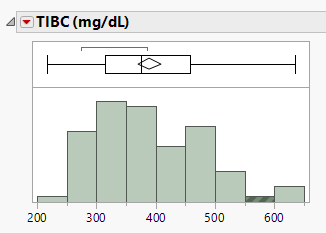
\includegraphics[width=0.6\linewidth]{Rozdzial3/decision}
		\caption{Przykłady rozkładu zmiennej decyzyjnej cz. 1}
		\label{fig:decision}
	\end{figure}

	\newpage
	\begin{figure}[!ht]
		\centering
		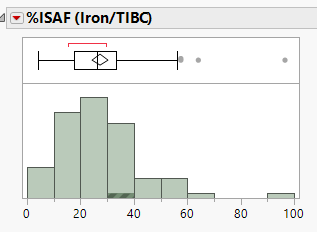
\includegraphics[width=0.6\linewidth]{Rozdzial3/decision1}
		\caption{Przykład rozkładu zmiennej decyzyjnej cz. 2}
		\label{fig:decision1}
	\end{figure}

	Pojedyncza zmienna - \textit{Gender} - posiada dychotomiczny charakter, aczkolwiek okazuje się relatywnie bardzo zrównoważona, posiadając rozkład na poziomie przynależności w 46,7\% do klasy F reprezentującej kobiety oraz 53,3\% do klasy M odpowiadającej mężczyznom. Rozkład tej zmiennej przedstawiono na rysunku \ref{fig:mnf}.
	
	\begin{figure}[!ht]
		\centering
		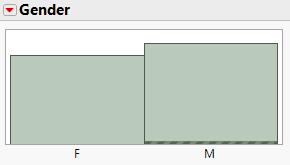
\includegraphics[width=0.6\linewidth]{Rozdzial3/mnf}
		\caption{Rozkład zmiennej Gender}
		\label{fig:mnf}
	\end{figure}
	
	\subsubsection{Czyszczenie i normalizacja rozkładu danych}
	
	W trakcie przeglądu obserwacji, zauważono pojedynczą obserwację z brakującą wartością zmiennej \textit{Ferritin}. Ze względu na wystąpienie tylko jednego takiego wpisu na 85 obserwacji, zdecydowano się na usunięcie jej. Pozostałymi kwestiami wymagającymi zaadresowania okazała się normalizacja rozkładu części zmiennych i decyzja o działaniu względem wartości odstających.
	
	W celu zmniejszenia ilości obserwacji odstających, postanowiono rozpocząć następny etap od problemu normalizacji rozkładu. Następujące zmienne, ze względu na ich obecną charakterystykę nie zostały poddane żadnym przekształceniom:
	
	\begin{enumerate}
		\item \textit{Age};
		\item \textit{Gender};
		\item \textit{TIBC}.
	\end{enumerate}

	Dla pozostałych zmiennych decyzyjnych zastosowano trzy rodzaje transformacji opisanych w sekcji omawiających dane klasyfikacyjne. Pierwszą z nich była obliczenie logarytmu z wartości zmiennej, które przyniosło zadowalający efekt dla zmiennych:
	
	\begin{enumerate}
		\item \textit{alpha GST};
		\item \textit{pi GST};
		\item \textit{sTfR};
		\item \textit{Ferritin} (zmienna odpowiedzi).
	\end{enumerate}

	Rysunek \ref{fig:log2} przedstawia przykład uzyskanej zmiany rozkładu dla zmiennej odpowiedzi.
	
	\begin{figure}[!ht]
		\centering
		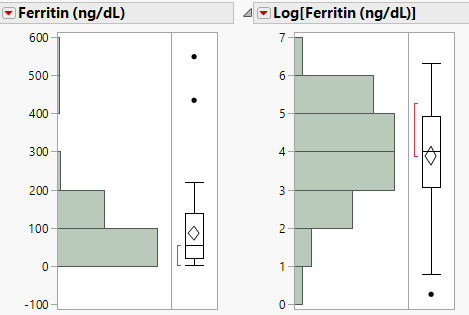
\includegraphics[width=0.7\linewidth]{Rozdzial3/log2}
		\caption{Wpływ transformacji logarytmicznej na rozkład zmiennej odpowiedzi}
		\label{fig:log2}
	\end{figure}

	Drugą transformacją o zadowalających wynikach okazało się zastosowanie pierwiastka kwadratowego, co pokazano na rysunku \ref{fig:cube2}. Wykorzystano ją do normalizacji rozkładu zmiennych:
	
	\begin{enumerate}
		\item \textit{Transferrin};
		\item \textit{Iron};
		\item \textit{\%ISAF}.
	\end{enumerate}

	\begin{figure}
		\centering
		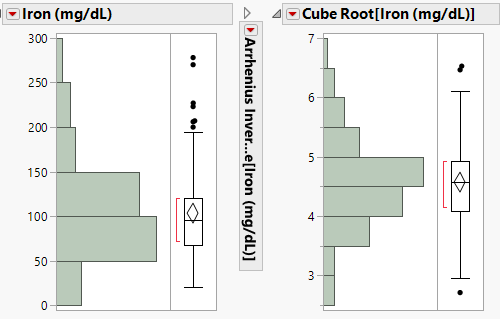
\includegraphics[width=0.7\linewidth]{Rozdzial3/cube2}
		\caption{Normalizacja rozkładu za pomocą transformacji pierwiastkiem kwadratowym.}
		\label{fig:cube2}
	\end{figure}

	Transformacja odwrotnym wzorem Arrheniusa okazała się nieskuteczna na wszystkich zmiennych, uzyskując gorsze efekty niż pozostałe przedstawione wyżej metody. Z racji na niewielką ilość obserwacji, oraz stosunkowo małą liczbę wartości odstających, zdecydowano się na pozostawienie ich do procesu uczenia. W celu kompatybilności z omawianymi bibliotekami, przekodowano zmienną dychotomiczną na wartości liczbowe.

\section{Szablony docelowych modeli dla zadanych danych eksperymentalnych}

W trakcie analizy zestawów danych wybrany został przedstawiony poniżej zestaw metod dla których wykonano i podsumowano testy praktyczne. Szablony struktury rozwiązań, takie jak np. wybór zmiennych uczestniczących w procesie uczenia, lub struktura sieci neuronowej zostały ustalone w sposób empiryczny z wykorzystaniem programu do uczenia maszynowego JMP. 

%\subsection{Regresja logistyczna}

%Badanie zależności w modelu regresji logistycznej odbyło się z wykorzystaniem wykresu wpływu zmiennej decyzyjnej na zmienną odpowiedzi opartego o p-wartość. Jako próg pozwalający na odrzucenie hipotezy zerowej (hipotezy o braku wypływu zmiennej na odpowiedź) przyjęto 0,05 jednostek. Rysunek \ref{fig:pvalue1} przedstawia w/w wykres wraz z p-wartościami dla poszczególnych zmiennych. Zauważyć można, że dla części zmiennych nie została wyznaczona p-wartość -- oznacza to, że część zmiennych jest ze sobą skorelowanych.

%Pierwszym krokiem w wybraniu istotnych zmiennych było usunięcie zmiennych skorelowanych, drugim natomiast stopniowe usuwanie zmiennych o p-wartości powyżej określonego progu. Rysunek \ref{fig:pvalue2} przedstawia listę wraz z wykresem kolumnowym istotnych regresorów. Ich lista, wraz z odpowiadającymi im p-wartościami została umieszczona w tabeli \ref{lin_reg:1}.

%\begin{table}
%	\centering
%	\begin{tabular}{l|c}
%		Nazwa zmiennej & p-wartość \\
%		\hline
%		\textit{Log mean largest texture} & 0,00000 \\
%		\textit{Log mean largest compactness} & 0,00000 \\
%		\textit{Cube root mean largest symmetry} & 0,00001 \\
%		\textit{Arrhenius inverse std err symmetry} & 0,00005 \\
%		\textit{Arrhenius inverse std err radius} & 0,00018 \\
%		\textit{Cube root mean concave points} & 0,00056 \\
%		\textit{Cube root mean largest concavity} & 0,00069 \\
%		\textit{Log std err texture} & 0,00252 \\
%		\textit{Cube root mean largest perimeter} & 0,00526 \\
%		\textit{Log mean smoothness} & 0,04867 \\
%		\textit{Log mean radius} & 0,04884
%	\end{tabular}
%	\caption{Lista istotnych regresorów}
%	\label{lin_reg:1}
%\end{table}

%\begin{figure}[!ht]
%	\centering
%	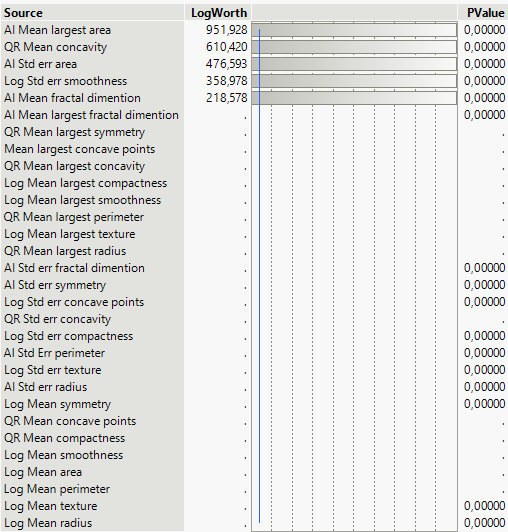
\includegraphics[width=0.9\linewidth]{Rysunki/Rozdzial3/pvalue1}
%	\caption{Wykres p-wartości dla całego zestawu zmiennych decyzyjnych.}
%	\label{fig:pvalue1}
%\end{figure}

%\newpage
%Dla wybranego zestawu zmiennych model osiągnął dokładność na poziomie $R^{2}$ = 0.9401. Zgodnie z macierzą pomyłek, 207 obserwacji typu \textit{Malignant} oraz 335 obserwacji \textit{Benign} zostało zaklasyfikowanych poprawnie. Oznacza to, że model uzyskał tylko 2 wyniki typu \textit{false-positive} (prawdopodobieństwo 0,6\%) i 5 wyników typu \textit{false-negative} (prawdopodobieństwo 2,4\%) dla danych treningowych. Ze względu na mały zestaw obserwacji, ryzyko przeuczenia jest znikome, w związku z czym nie wytypowano zestawu danych walidacyjnych. Rysunek \ref{fig:roc} przedstawia krzywą charakterystyczną odbiornika dla modelu. 

%\begin{figure}[!ht]
%	\centering
%	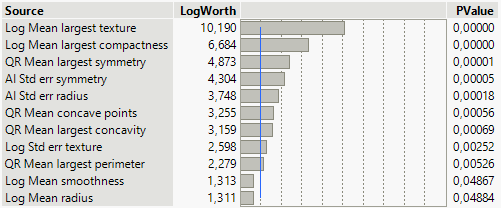
\includegraphics[width=0.7\linewidth]{Rysunki/Rozdzial3/pvalue2}
%	\caption{Wykres i p-wartości istotnych zmiennych decyzyjnych}
%	\label{fig:pvalue2}
%\end{figure}

%\begin{figure}[!ht]
%	\centering
%	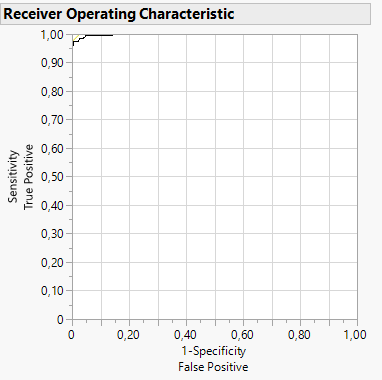
\includegraphics[width=0.5\linewidth]{Rysunki/Rozdzial3/roc}
%	\caption{Krzywa charakterystyczna odbiornika (ROC) dla modelu regresji logistycznej}
%	\label{fig:roc}
%\end{figure}

%\subsection{Głęboka sieć neuronowa}

%Do przygotowania sieci neuronowej wykorzystano zestaw zmiennych zawartych w tabeli \ref{lin_reg:1}. Dane zostały losowo podzielony na dane uczące i walidacyjne w propocji 80\% do 20\%. W wyniku prób i błędów, optymalny model uzyskano przy strukturze przedstawionej w tabeli \ref{neural:1}. Graficzny schemat struktury został także przedstawiony na rysunku \ref{fig:neuralstruct}.

%\begin{table}[!ht]
%	\centering
%	\begin{tabular}{c|c|c}
%		Typ warstwy & ilość neuronów & aktywacja \\
%		\hline
%		ukryta & 5 & tangens hiperboliczny \\
%		ukryta & 5 & tangens hiperboliczny \\
%		wyjściowa & 2 & ---	
%	\end{tabular}
%	\caption{Struktura modelu sieci neuronowej}
%	\label{neural:1}
%\end{table}

%\begin{figure}[!ht]
%	\centering
%	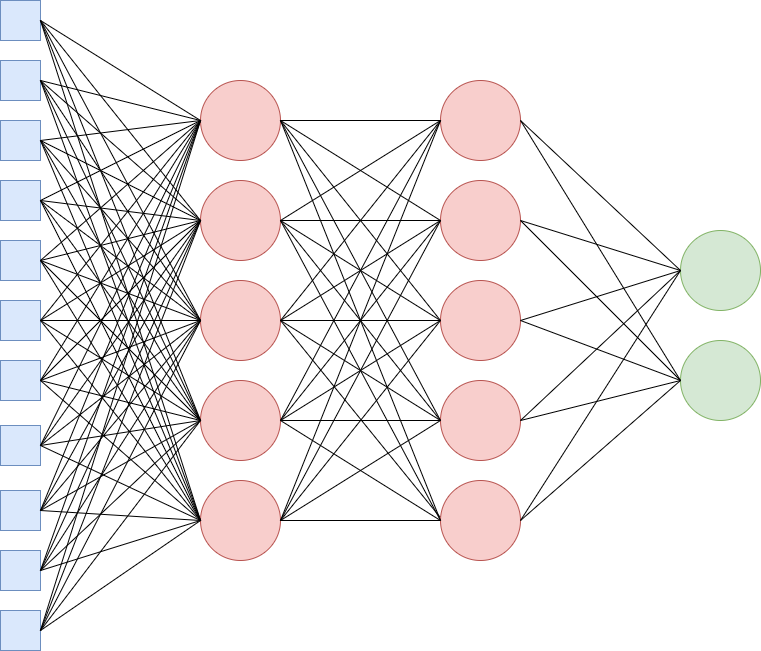
\includegraphics[width=0.6\linewidth]{Rysunki/Rozdzial3/neural_struct}
%	\caption{Schemat struktury sieci}
%	\label{fig:neuralstruct}
%\end{figure}

%Środowisko JMP nie udostępnia informacji o funkcji aktywacji warstwy wyjściowej, w związku z czym w tabeli 3.2 została ona pominięta. Dla ziarna o wartości 1234 uzyskano model którego statystyka $R^{2}$ dla danych treningowych wyniosła 0.966268, natomiast dla danych testowych 0.9924547. Trafność dla losowo wybranego zestawu testowego wyniosła 100\%, natomiast dla danych uczących napotkano 5 przypadków \textit{false-negative} (prawdopodobieństwo 3\%) oraz 1 przypadek \textit{false-positive} (prawdopodobieństwo 0,4\%). Rysunki \ref{fig:roctest} oraz \ref{fig:rocvalid} przedstawiają krzywe charakterystyczne odbiornika dla zestawu testowego i walidacyjnego.

%\begin{figure}[!ht]
%	\begin{minipage}{0.48\textwidth}
%			\centering
%			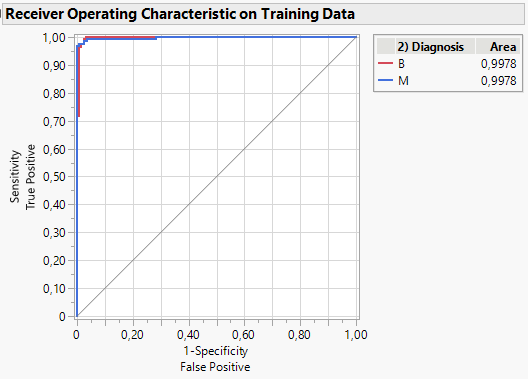
\includegraphics[width=0.95\linewidth]{Rysunki/Rozdzial3/roc_test}
%			\caption{Krzywa charakterysty-czna odbiornika dla zestawu testowego}
%			\label{fig:roctest}
%	\end{minipage}%
%	\hspace{8pt}
%	\begin{minipage}{0.48\textwidth}
%			\centering
%			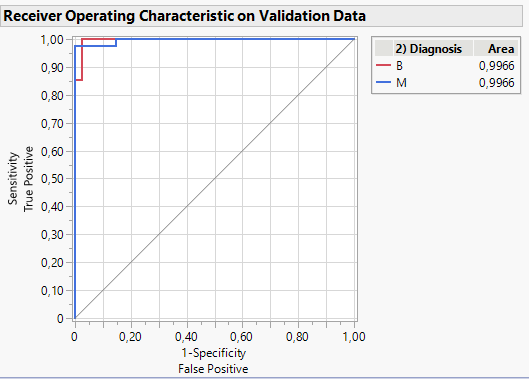
\includegraphics[width=0.95\linewidth]{Rysunki/Rozdzial3/roc_valid}
%			\caption{Krzywa charakterysty-czna odbiornika dla danych walidacyjnych}
%			\label{fig:rocvalid}
%	\end{minipage}
%\end{figure}

\subsection{Maszyna wektorów nośnych}

Do predykcji diagnozy wykorzystano ten sam zestaw regresorów, zawartych w tabeli 3.1. Ponownie w celu walidacji użyto metody wybrania losowego zestawu walidacyjnego spośród dostarczonych danych, w proporcji 80\% obserwacji uczących i 20\% testowych, z użyciem wartości 1234 dla ziarna generatora liczb pseudolosowych. Jako funkcję jądra maszyny wektorów nośnych (ang. Support Vector Machine, SVM) wybrano \textit{Radial Basis Function}, która jest domyślnym wyborem dla SVM w środowisku JMP. 

\begin{longtable}{l | c}
	\centering
	Zmienna decyzyjna & wartość X \\
	\hline
	\textit{Log mean largest texture} & 3,217 \\
	\textit{Log mean largest compactness} & -1,5504 \\
	\textit{Cube root mean largest symmetry} & 0,65891 \\
	\textit{Arrhenius inverse std err symmetry} & 635100 \\
	\textit{Arrhenius inverse std err radius} & 38170 \\
	\textit{Cube root mean concave points} & 0,33665 \\
	\textit{Cube root mean largest concavity} & 0,5951 \\
	\textit{Log std err texture} & 0,1049 \\
	\textit{Cube root mean largest perimeter} & 4,7045 \\
	\textit{Log mean smoothness} & -2,3502 \\
	\textit{Log mean radius} & 2,6191 \\
	\caption{Wartości składowych X modelu dla poszczególnych zmiennych decyzyjnych}
	\label{svm:1}
\end{longtable} 

\begin{figure}[!ht]
	\begin{minipage}{0.48\textwidth}
		\centering
		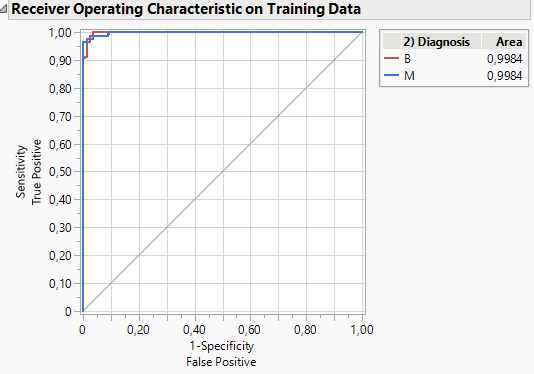
\includegraphics[width=0.98\linewidth]{Rysunki/Rozdzial3/roc_svm1_test}
		\caption{Krzywa charakterystycz-na odbiornika dla danych uczących modelu SVM}
		\label{fig:rocsvm1test}		
	\end{minipage}%
	\hspace{10pt}
	\begin{minipage}{0.48\textwidth}
		\centering
		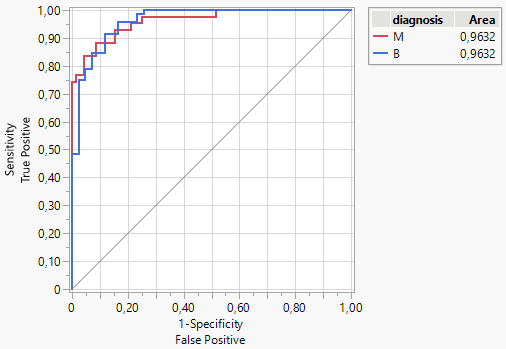
\includegraphics[width=0.98\linewidth]{Rysunki/Rozdzial3/roc_svm1_val}
		\caption{Krzywa charakterystycz-na odbiornika dla danych walidacyjnych modelu SVM}
		\label{fig:rocsvm1val}				
	\end{minipage}	
\end{figure}

Utworzony w ten sposób model posiada generalizowaną statystykę $R^{2}$ na poziomie 0.97161 dla zestawu walidacyjnego, i uzyskał wskaźnik błędnej klasyfikacji wynoszący 0\% dla danych testowych, oraz 1,3\% dla danych uczących. Tabela \ref{svm:1} przedstawia wartości X dla poszczególnych regresorów. Rysunki \ref{fig:rocsvm1test} oraz \ref{fig:rocsvm1val} przedstawiają krzywe charakterystyczne odbiornika dla uzyskanego modelu, pola pod którymi uzyskały wartość odpowiednio 0,9984 dla danych uczących i 1 dla danych testowych.

\subsection{Regresja liniowa}

Podobnie jak w przypadku regresji logistycznej, do ustalenia które z regresorów mają największy wpływ na zmienną odpowiedzi zastosowano wykres wpływu poszczególnych zmiennych oparty o p-wartość. Jako próg zaakceptowania parametru do procesu uczenia zdecydowano się na wybranie p-wartości wynoszących poniżej 0,05 jednostek. Rysunek \ref{fig:pvalue3} przedstawia wykres dla wszystkich zmiennych, natomiast rysunek \ref{fig:pvalue4} ukazuje wykres zawierający jedynie wybrane zmienne. 

\begin{figure}[!ht]
	\centering
	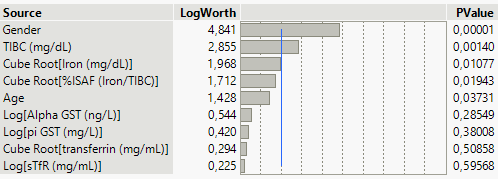
\includegraphics[width=\linewidth]{Rozdzial3/pvalue3}
	\caption{Wykres p-wartości dla wszystkich zmiennych}
	\label{fig:pvalue3}
\end{figure}

\begin{figure}[!ht]
	\centering
	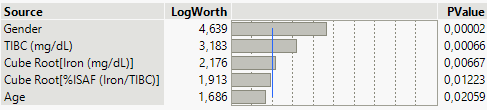
\includegraphics[width=\linewidth]{Rozdzial3/pvalue4}
	\caption{Wykres p-wartości dla zmiennych wybranych do procesu uczenia}
	\label{fig:pvalue4}
\end{figure}

W procesie eliminacji regresorów o p-wartości przekraczającej wybrany próg akceptacji, wybrano następujące zmienne do procesu uczenia:

\begin{table}[!ht]
	\begin{minipage}{0.48\textwidth}
		\centering
		\begin{tabular}{l|c}
			Nazwa zmiennej & p-wartość \\
			\hline
			\textit{Gender} & 0.00002 \\
			\textit{TIBC} & 0.00066 \\
			\textit{Cube Root Iron} & 0.00667 \\
			\textit{Cube Root \%ISAF} & 0.01223 \\
			\textit{Age} & 0.02059
		\end{tabular}
		\caption{Wybrane zmienne decyzyjne i ich p-wartości}
		\label{pvalue}
	\end{minipage}%
	\hspace{0.04\textwidth}
	\begin{minipage}{0.48\textwidth}
		\centering
		\begin{tabular}{l|c}
			Nazwa zmiennej & waga \\
			\hline
			\textit{Intercept} & 8,498959 \\
			\textit{Age} & 0.0201022 \\
			\textit{Gender[F - M]} & -0.959795 \\
			\textit{Cube Root Iron} & 2,9461861 \\
			\textit{TIBC} & -0.014182 \\
			\textit{Cube Root \%ISAF} & -4,356345
		\end{tabular}
		\caption{wartości wag zmiennych decyzyjnych}
		\label{weights}		
	\end{minipage}
\end{table}

W wyniku uczenia uzyskano model którego wartość metryki \textit{$R^2$} wyniosła 0.4654525, co sugeruje że dane są słabo aproksymowalne liniowo. Tabela \ref{weights} przedstawia nauczone wagi poszczególnych regresorów.
\chapter{Biblioteka TensorFlow}

\section{Wprowadzenie}

Tnesorflow to darmowa biblioteka do uczenia maszynowego typu \textit{open-source} stworzona przez Google. Oferuje ona możliwość przeprowadzenia płytkiego oraz głębokiego uczenia maszynowego, z wykorzystaniem własnych lub gotowych zestawów danych. Pozwala ona także na użycie pretrenowanych modeli jako rozwiązanie docelowe lub część składowa własnego modelu. Stanowi ona jedną z najpopularniejszych bibliotek ML, w szczególności wśród osób dopiero rozpoczynające swoje doświadczenia z tą gałęzią informatyki.

Jak podano na stronie domowej biblioteki Tensorflow\cite{tf}, deklaruje ona bycie odpowiednią zarówno do przeprowadzania badań, jak i do wykorzystania w zastosowaniach przemysłowych. W momencie pisania niniejszej pracy, najnowszą dostępną wersją jest Tensorflow 2.11.

\section{Metody wdrożenia modeli}

Biblioteka umożliwia następujące metody wdrożenia modeli dla języka C++ \cite{protobuf}\cite{deploy3}\cite{tflite}:

\begin{itemize}
	\item API TensorFlow w języku C++
	\item Środowisko wykonawcze ONNX
	\item Zestaw narzędzi TensorFlow Lite
	\item Za pomocą Protobuf
\end{itemize}

\subsection{API w języku C++}

Z racji bycia napisanym w języku C++, biblioteka TensorFlow oferuje wsparcie do tworzenia, ternowania, i wdrażania modeli uczenia maszynowego w tym języku, poprzez udostępnienie użytkownikom interfejsu programowania aplikacji (ang. \textit{Application Programming Interface, API}). Udostępnia ono operacje pozwalające manipulacje tensorami, wykonywanie operacji matematycznych na tensorach i ich elementach, budowę modelu w postaci grafu obliczeniowego, oraz jego uruchomienia wykorzystując różne metody obliczeniowe, np. Adagrad oraz metodę spadku gradientowego \cite{tfcpp}. Zastosowanie tego API pozwala na utworzenie i pracę z modelem bezpośrednio w aplikacji pisanej w języku C++.

\cppcode{Rozdzial4/helloworldgraph.cpp}{Przykład utworzenia grafu obliczeniowego w TensorFlow realizującego konkatenację ciągów znakowych \cite{tfhelloworld}}

\subsection{Środowisko wykonawcze ONNX}

\textit{Open Neural Networks Exchange, (ONNX)} to środowisko mające na celu standaryzację reprezentacji modeli uczenia maszynowego, autorstwa firmy Microsoft \cite{deploy3}. Pozwala ono na uniezależnienie modelu na etapie wdrożenia od biblioteki i języka w którym został stworzony, pozwalając na ich użycie przy pomocy pojedynczego mechianizmu. Wykorzystanie tej metody wdrażania modeli polega na przygotowaniu ich za pomocą API języka okraz eksport do struktury akceptowanej przez środowisko wykonawcze ONNX.

\subsection{Zestaw narzędzi TensorFlow Lite}

Stanowi zbiór narzędzi (ang. \textit{toolbox}) umożliwiających uruchomienie przygotowanych modeli na platformach mobilnych oraz urządzeniach brzegowych (takich jak moduły IoT, lub ogólnie rozumiane systemy mokroprocesorowe). Pozwala on dodatkowo m.in. na wykorzystanie akceleracji sprzętowej oraz optymalizacji modelu. Przygotowywanie modeli do uruchomienia za pomocą tej metody na wybranej platformie składa się m.in. z przygotowania modelu z użyciem biblioteki TensorFlow Lite Model Maker, wykorzystania jednego z gotowych, pretrenowanych modeli, lub konwersji modelu TensorFlow z formatu protobuf \cite{tflite}.

\subsection{Za pomocą Protobuf}

Utworzony w bibliotece TensorFlow model jest zapisywany do formatu wykorzystywanego przez mechanizm Protocol Buffers autorstwa Google, zwanego potocznie \textit{Protobuf}. Pozwala on na przechowywanie grafu obliczeniowego modelu w notacji niezależnej od języków programowania, z której następnie narzędzie Protobuf umożliwia wygenerowanie odpowiednich klas i struktur danych dla wybranego języka, jak np. C++ czy Python \cite{protobuf2}. Pliki Protobuf mogą mieć formę tekstową, która ułatwia edycję i analizę człowiekowi, lub formę binarną, pozwalającą na znaczne zaoszczędzenie miejsca w przypadku przechowywania danych numerycznych, jak np. wagi połączeń sieci. 

\cppcode{Rozdzial4/cppconstructor.cpp}{Konstruktor klasy \textit{Model} odczytujący strukturę modelu z pliku Protobuf \cite{input_tf}}

\section{Formaty źródeł danych}

W języku C++ biblioteka TensorFlow wymaga podania danych w postaci obiektów klasy szablonowej \textit{std::vector} z biblioteki STL języka \cite{input_tf}, lub za pomocą własnych klas, np. \textit{FeedDict}, jednak nie określa w jaki sposób muszą te dane być przechowywane. W związku z tym, możliwe jest wykorzystanie dowolnego formatu przechowywania danych do uczenia, pod warunkiem zapewnienia mechanizmu ich parsowania. Typ przechowywany przez obiekty std::vector zależny jest od ilości regresorów, i może przyjmować postać typu prostego lub złożonego. Dane powinny być rozgraniczone przed procesem uczenia na dwa wektory, z których jeden przechowuje dane uczące, natomiast drugi dane walidacyjne.

\cppcode{Rozdzial4/tfruntrainingstep.cpp}{Przykładowa funkcja realizująca krok uczenia \cite{input_tf}}

\section{Metody przetwarzania i eksploracji danych}

API biblioteki TensorFlow dla języka C++ oferuje wiele operacji możliwych do wykonania na danych wykorzystywanych do uczenia. Operacje te można podzielić na manipulujące strukturą zapisanych danych (pozwalające na przetworzenie tensorów lub optymalizację pracy z danymi), oraz manipulujące wartościami regresorów (jak np. operacje matematyczne). Poniżej wymieniono wybrane, szczególnie istotne funkcjonalności przetwarzania i eksploracji danych, wyszczególnione w dokumentacji \cite{tfcpp}:

\subsection{Operacje strukturalne}

Są to operacje mające na celu modyfikację struktury w jakich przechowywane są dane. Biblioteka oferuje szereg funkcjonalności mających na celu reformatowanie danych w celu optymalizacji wykonywania na nich obliczeń\cite{tfcpp}. Należą do nich:

\begin{itemize}
	\item \textbf{bitcast} - zmiana typu tensora bez kopiowania danych;
	\item \textbf{dekwantyzacja} - zamiana na typ zmiennoprzecinkowy z formatu stałoprzecinkowego lub całkowitoliczbowej notacji wykładniczej;
	\item \textbf{udawana kwantyzacja} - wykorzystywana do przygotowania danych aby móc z nich obliczyć gradient (dostępne jest kilka rodzajów udawanej kwantyzacji);
	\item \textbf{padding} - otoczenie wartości tensora nadmiarowymi wartościami w celu dostosowania wymiarów (możliwe uzupełnienie np. zerami, lub wartościami lustrzanymi);
	\item \textbf{stacking} - złącza N tensorów R-wymiarowych w jeden tensor R+1-wymiarowy;
	\item \textbf{dynamic stitching i partitioning} - złączanie danych z wielu tensorów w jeden lub rozdzielanie z jednego na wiele;
	\item \textbf{serializacja} - konwersja tensora na serializowany format dla Protobuf.
\end{itemize}

\subsection{Eksploracja danych}

W dokumentacji API TensorFlow dla C++ możliwe jest znalezienie wielu operacji pozwalających manipulować wartościami danych w celu wyliczenia pewnych cech, lub dokonania obliczeń potrzebnych w trakcie procesu uczenia\cite{tfcpp}. Do najistotniejszych z nich należą:

\begin{itemize}
	\item wyliczanie odcisku palca danych (ang. \textit{fingerprint});
	\item weryfikacja czy dane zawierają wartości NaN lub inf;
	\item wyodrębnienie fragmentów obrazów do warstwy ,,depth'';
	\item obliczenie gradientu z danych po udawanej kwantyzacji;
	\item obliczanie rzadkiego (ang. \textit{sparse}) gradientu dla danego akumulatora;
	\item obliczenie odwrotnej permutacji tensora;
	\item normalizacja za pomocą kwantyzacji;
	\item wybór kandydatów do ewaluacji funkcji wyjściowych (ang. \textit{candidate sampling});
	\item dostosowywanie nasycenia, kontrastu i kolorystyki obrazów;
	\item dekodowanie obrazów z różnych formatów (np. gif, bmp, jpg, bmp);
	\item dekodowanie danych z różnych źródeł (np. csv, json);
	\item generowanie ramek (ang. \textit{bounding box});
	\item zmiana rozmiaru obrazów;
	\item rekodowanie obrazu z kolorystyki RGB na HSV;
	\item zachłanna selekcja ramek;
	\item różnorodne operacje matematyczne;
	\item pooling i konwoolucję;
	\item normalizację z pomocą gradientów;
	\item różnorodne funkcje aktywacji i straty;
	\item operacje na ciągach znakowych;
	\item algorytmy treningowe, jak np. Adagrad, Adadelta, centered RMSProp.
	
\end{itemize}

\subsection{Sterowanie przepływem obliczeń}

Oprócz wymienionych wcześniej poleceń optymalizujących lub przetwarzających dane, biblioteka TensorFlow posiada szereg operacji zarządzających przepływem danych w grafie obliczeniowym reprezentującym model. Należą do nich:

\begin{itemize}
	\item operacje na zakumulowanych gradientach;
	\item ustawianie barier;
	\item operacje na mapach, kolejkach i tablicach tensorów.
	
\end{itemize}

\section{Modele uczenia maszynowego}

Bazując na informacjach dostępnych w dokumentacji API biblioteki TensorFlow dla języka C++, w chwili obecnej udostępnia ono głównie funkcjonalności związane z sieciami neuronowymi. Możliwe do zbudowania z ich wykorzystaniem modele to:

\begin{itemize}
	\item jednokierunkowa sieć neuronowa (ang. \textit{feedforward neural network});
	\item splotowa sieć neuronowa;
	\item rekurencyjna sieć neuronowa;
	\item autoenkodery;
	\item wzmocnione uczenie maszynowe;
\end{itemize}

Powyższe modele mogą zostać wykorzystane do rozwiązywania wielu problemów, w tym także o charakterystyce liniowej czy klasyfikacji. Szczególnie istotne z punktu widzenia biostatystyki może być model rekurencyjnej oraz jednokierunkowej sieci, który pozwala na analizę danych numerycznych, i jest relatywnie prosty w zrozumieniu sposobu działania, ze względu na analogię do funkcjonowania neuronów w ludzkim mózgu.

\subsection{Przykład jednokierunkowej sieci neuronowej}

PARSOWANIE CSV

UTWORZENIE MODELU

TRENING MODELU

\section{Metody analizy modeli}
\section{Dostępność dokumentacji i źródeł wiedzy}
\chapter{Biblioteka Shark-ML}

\section{Wprowadzenie}

Shark-ML to biblioteka uczenia maszynowego dedykowana dla języka C++. Posiada ono otwarte źródło, i udostępniana jest na podstawie licencji \textit{GNU Lesser General Public License}. Głównymi aspektami na których skupia się ta biblioteka są problemy liniowej i nieliniowej optymalizacji (w związku z czym posiada ona część funkcjonalności biblioteki do algebry liniowej), maszyny jądra (np. maszyna wektorów nośnych) i sieci neuronowe. \cite{shark} Podmiotami udostępniającymi bibliotekę jest Uniwersytet Kopenhagi w Danii, oraz Instytut Neuroinformatyki z Ruhr-Universitat Bochum w Niemczech.

\section{Formaty źródeł danych}

Biblioteka operuje na własnych reprezentacjach macierzy i wektorów, które tworzone są poprzez opakowywanie surowych tablic za pomocą specjalnych adapterów, jak np. \textit{remora::dense\char`_matrix\char`_adaptor<>()} lub za pomocą kontenerów biblioteki standardowej C++ i funkcji \textit{createDataFromRange()}. Mechanizm ten jest identyczny jak w przypadku pozostałych z omawianych bibliotek, co daje użytkownikowi dużą dowolność co do sposobu przechowywania danych i mechanizmu ich odczytywania. Posiada ona także dedykowany parser dla plików w formacie CSV, lecz zakłada on obecność w pliku jedynie danych numerycznych. Do jego użycia należy użyć klasy kontenera \textit{ClassificationDataset} lub \textit{RegressionDataset} oraz metody \textit{importCSV} która zapisuje odczytane dane do wcześniej wspomnianego obiektu poprzez mechanizm zwracania przez parametr. Jeden z argumentów funkcji określa która z kolumn zawiera zmienną decyzyjną, dzięki czemu biblioteka jest w stanie od razu oddzielić dane wejściowe od kolumny oczekiwanych wartości. Artykuł ,,Classification with Shark-ML machine learning library''\cite{shark:http} dostępny na platformie GitHub pokazuje także, jak pobrać dane w postaci formatu CSV z internetu z pomocą API biblioteki \textit{curl}, i przetworzyć je do formy akceptowanej przez Shark-ML. W aktualnej wersji biblioteki znalazły się także wbudowane funkcje pobierania danych współpracujące z protokołem HTTP. Listing \ref{shark:csv} ukazuje jak odczytać dane z pliku .csv znajdującego się na dysku użytkownika.

\newpage
\cppcode{Result/inc/shark/csv.hpp}{Odczytanie danych z pliku CSV}{shark:csv}

W celu opakowania danych zawartych w kontenerach biblioteki standardowej języka C++ do obiektów akceptowanych przez bibliotekę Shark-ML, konieczne jest wykorzystanie specjalnych funkcji adaptorowych, do których przekazywany jest wskaźnik na dane w postaci surowej tablicy, wraz z oczekiwanymi wymiarami wynikowej macierzy / wektora. Sposób opakowania danych pokazano na listingu \ref{shark:adaptor}

\cppcode{Rozdzial5/shark-adaptor.cpp}{Sposób opakowywania danych do przetwarzania przez Shark-ML \cite{handsOnMachineLearning}}{shark:adaptor}

\section{Metody przetwarzania i eksploracji danych}

\subsection{Normalizacja}

Biblioteka Shark-ML implementuje normalizacje jako klasy treningowe dla modelu \textit{Normalizer}, udostępniając użytkownikowi trzy możliwe do wykorzystania klasy:

\begin{itemize}
	\item \textit{NormalizeComponentsUnitInterval} - przetwarza dane tak aby mieściły się w przedziale jednostkowym;
	\item \textit{NormalizeComponentsUnitVariance} - przelicza dane aby uzyskać jednostkową wariancję, i niekiedy także średnią wynoszącą 0.
	\item \textit{NormalizeComponentsWhitening} - dane przetwarzane są w sposób zapewniający średnią wartość wynoszącą zero oraz określoną przez użytkownika wariancję (domyślnie wariancja jednostkowa).
\end{itemize}

Opierają się one o użycie metody \textit{train()} na obiekcie normalizera, aby odpowiednio go skonfigurować do przetwarzania zarówno danych testowych, jak i wszystkich innych danych które użytkownik ma zamiar wprowadzić do modelu. Dodatkowymi funkcjami jest możliwość przemieszania danych, i wydzielenia fragmentu jako dane testowe za pomocą metody \textit{shuffle()} klasy \textit{ClassificationDataset} oraz funkcji \textit{splitAtElement()}. Listing \ref{shark:http} pokazuje przykład wstępnego przetwarzania danych z wykorzystaniem normalizacji.

\cppcode{Result/inc/shark/normalization.hpp}{Wstępne przetwarzanie danych do uczenia \cite{shark:http}}{shark:preprocessing}

\subsection{Redukcja wymiarowości}
\subsubsection{PCA}
Algorytm redukcji wymiarowości PCA implementowany jest w bibliotece Shark za pośrednictwem klasy \textit{PCA}. Wykorzystuje ona obiekt modelu liniowego w formie enkodera oraz przyjmuje oprócz niego w metodzie \textit{encoder} docelowy wymiar zestawu danych. Wynikiem działania wymienionej metody jest konfiguracja modelu liniowego do tworzenia zestawu danych o zredukowanym wymiarze. Listing \ref{shark:pca} przedstawia sposób wykorzystania klasy PCA.

\cppcode{Rozdzial5/shark-dimension-reduction.cpp}{Redukcja wymiarowości danych z wykorzystaniem klasy PCA i enkodera}{shark:pca}


\subsubsection{Liniowa analiza dyskryminacyjna}

Liniowa analizy dyskryminacyjnej (ang. \textit{Linear Discriminant Analysis, LDA}) w przypadku biblioteki Shark-ML opiera się o rozwiązanie analityczne, poprzez konfigurację klasy modelu \textit{LinearClassifier} przez klasę treningową \textit{LDA}, wykorzystując funkcję \textit{train()}. Możliwe jest także wykorzystanie LDA do zadania klasyfikacji, uzyskując predykcje dla zestawu danych za pomocą wywołania obiektu liniowego klasyfikatora jak funkcji (użycie operatora ()) przekazując mu dane uzyskane z ClassificationDataset za pomocą metody \textit{inputs()}. Szczegóły implementacyjne dla redukcji wymiarowości danych zamieszczone zostały na listingu \ref{shark:lda-red}, natomiast listing \ref{shark:lda} przedstawia sposób użycia LDA do zadania klasyfikacji.

\cppcode{Rozdzial5/shark-lda-red.cpp}{Przykład redukcji zestawu danych z wykorzystaniem modelu LDA \cite{handsOnMachineLearning}}{shark:lda-red}

\subsection{Regularyzacja L1}

Biblioteka Shark, w przeciwieństwie do Shogun nie posiada ściśle określonych mechanizmów regularyzacji dla danych metod uczenia maszynowego. Zamiast tego, istnieje możliwość umieszczenia obiektu wykonującego regularyzację w obiekcie klasy trenera, za pomocą metody \textit{setRegularization()}. W celu zastosowania metody Lasso, należy umieścić w wybranym trenerze obiekt klasy \textit{shark::OneNormRegularizer}, a następnie przeprowadzić proces uczenia.

\subsection{Regularyzacja L2}

Podobnie jak w przypadku metody Lasso, wykorzystanie regularyzacji L2 w trenowanym modelu opiera się na wstrzyknięciu obiektu regularyzatora do obiektu klasy trenera. Dla metody L2 jest to obiekt klasy \textit{shark::TwoNormRegularizer}.


\section{Modele uczenia maszynowego}

\subsection{Regresja liniowa}

Jednym z podstawowych modeli oferowanych przez niniejszą bibliotekę jest regresja liniowa. Do celów jej reprezentacji dostępna jest klasa \textit{LinearModel}, oferująca rozwiązanie problemu w sposób analityczny za pomocą klasy trenera \textit{LinearRegression}, lub podejście iteracyjne implementowane przez klasę trenera \textit{LinearSAGTrainer}, wykorzystujące iteracyjną metodę gradientu średniej statystycznej (ang. \textit{Statistic Averagte Gradient, SAG}). W przypadku bardziej skompilowanych regresji, gdzie może nie istnieć rozwiązanie analityczne, istnieje możliwość zastosowania podejścia iteracyjnego z użyciem optymalizatora wybranego przez użytkownika. Metoda ta sprowadza się to uczenia optymalizatora z wykorzystaniem funkcji straty, a następnie załadowanie uzyskanych wag do modelu regresji. Parametry modelu możliwe są do odczytania z wykorzystaniem metod \textit{offset()} i \textit{matrix()} lub metody \textit{parameterVector()}. Na listingu \ref{shark:linear} ukazane zostało wykorzystanie podejścia iteracyjnego, natomiast listing \ref{shark:linear2} przedstawia metodę analityczną.

\cppcode{Result/inc/shark/linear.hpp}{Przykład regresji liniowej z wykorzystaniem optymalizatora spadku gradientowego}{shark:linear}

\cppcode{Rozdzial5/shark-linear2.cpp}{Przykład regresji liniowej z wykorzystaniem trenera analitycznego \cite{handsOnMachineLearning}}{shark:linear2}

\subsection{Regresja logistyczna}

Mechanizm regresji logistycznej dostępny w bibliotece Shark-ML z natury rozwiązuje problem regresji binarnej. Istnieje jednak możliwość przygotowania wielu klasyfikatorów, w ilości wyrażonej wzorem:

\begin{equation}
	\frac{N(N-1)}{2}	
	\label{multiclass}
\end{equation}

gdzie N oznacza ilość klas występujących w problemie. Utworzone klasyfikatory następnie są złączane w jeden za pomocą odpowiedniej konfiguracji obiektu \textit{OneVersusOneClassifier}, rozwiązując problem klasyfikacji wieloklasowej. W tym celu zestaw danych należy iteracyjnie podzielić na podproblemy o charakterystyce binarnej za pomocą wbudowanej funkcji \textit{binarySubProblem()} przyjmującej zestaw danych i klasy. Nauczanie poszczególnych modeli realizowane jest poprzez klasę trenera \textit{LogisticRegression}. Po zakończeniu trenowania okreslonej partii pomniejszych modeli, są one ładowane do głównego modelu. Wykorzystanie gotowego klasyfikatora wieloklasowego nie różni się od sposobu użycia modelu uzyskanego np. w klasyfikacji liniowej. Listing \ref{shark:logistic} prezentuje funkcję budującą model logistycznej regresji wieloklasowej, natomiast listing \ref{shark:logistic2} pokazuje sposób utworzenia prostego modelu dla problemu binarnego.

\cppcode{Rozdzial5/shark-logistic.cpp}{Przykład funkcji tworzącej model wieloklasowej regresji logistycznej \cite{handsOnMachineLearning}}{shark:logistic}

\cppcode{Result/inc/shark/logistic.hpp}{Przykład prostej binarnej regresji logistycznej}{shark:logistic2}

\subsection{Maszyna wektorów nośnych}

Jednym z bardzo istotnych z perspektywy zastosowania biblioteki Shark-ML oferowanych przez nią metod uczenia maszynowego jest maszyna wektorów nośnych stanowiąca rodzaj tzw. modeli jądra (ang. \textit{kernel model}). Opiera się ona na wykonaniu regresji liniowej w przestrzeni cech określonych przez wykorzystany kernel. Podobnie jak w przypadku regresji logistycznej, API biblioteki umożliwia wykonanie klasyfikacji dla przypadku binarnego, natomiast rozwiązanie przy jej użyciu problemu wieloklasowego wymaga kombinacji instancji maszyn wektorów nośnych w model złożony, czego można dokonać przy pomocy klasy \textit{OneVersusOneClassifier} oraz ilości klas wyrażonej wzorem \ref{multiclass}. Zgodnie z charakterystyczną cechą tej biblioteki, użycie metody podzielone jest na utworzenie instancji modelu oraz obiektu klasy trenera, która go konfiguruje w procesie uczenia. W tym celu dostępne są dla użytkownika klasy:

\begin{itemize}
	\item \textit{GaussianRbfKernel} - odpowiada za obliczenie podobieństwa między zadanymi cechami wykorzystując funkcję bazową \textit{ang. Radial Basis Function, RBF};
	\item \textit{KernelClassifier} - funkcja realizująca regresję liniową wewnątrz przestrzeni określonej przez jądro;
	\item \textit{CSvmTrainer} - klasa trenera realizująca uczenie w oparciu o skonfigurowane parametry;
\end{itemize}

Do parametrów pozwalających na konfigurację modelu należą m.in.:

\begin{itemize}
	\item przepustowość modelu - podawana w konstruktorze \textit{GaussianRbfKernel} jako liczba z przedziału $\langle 0 ; 1 \rangle$;
	\item regularyzacja - podawana jako liczba rzeczywista w konstruktorze \textit{CSvmTrainer}, domyślnie maszyna wektorów nośnych używa kary typu \textit{1-norm penalty} za przekroczenie docelowej granicy;
	\item bias - flaga binarna (bool) określająca czy model ma używać biasu, podawana w konstruktorze \textit{CSvmTrainer};
	\item \textit{sparsify} - parametr określający czy model ma zachować wektory które nie są nośne, dostępny przez metodę \textit{sparsify()} trenera;
	\item minimalna dokładność zakończenia nauczania - pozwala wyspecyfikować precyzję modelu, jest dostępna jako pole struktury zwracane przez metodę \textit{stoppingCondition()} klasy trenera;
	\item wielkość cache - ustawiana za pomocą funkcji \textit{setCacheSize()} trenera;
\end{itemize}

Sposób użycia modelu jest identyczny jak w przypadku pozostałych modeli, poprzez operator wywołania funkcji - (). Listing \ref{shark:svm} ukazuje przykład utworzenia i skonfigurowania modelu na podstawie wpisów dostępnych w dokumentacji biblioteki, natomiast listing \ref{shark:svm} przedstawia sposób utworzenia maszyny wektorów nośnych dla problemów wieloklasowych wewnątrz funkcji przyjmującej zestawy danych uczących i testowych.

\cppcode{Result/inc/shark/svm.hpp}{Przykład maszyny wektorów nośnych dla problemu binarnego}{shark:svm}

\cppcode{Rozdzial5/shark-svm2.cpp}{Przykład maszyny wektorów nośnych dla problemu wieloklasowego \cite{handsOnMachineLearning}}{shark:svm2} 

\subsection{Algorytm K najbliższych sąsiadów}

Jedną z metod klasyfikacji oferowanych przez bibliotekę Shark-ML jest model najbliższych sąsiadów, który można wyposażyć w różne algorytmy, w tym w algorytm kNN (ang. \textit{K Nearest Neighbours}). Do reprezentacji modelu stworzona została klasa \textit{NearestNeighborModel}. Biblioteka umożliwia wykorzystanie rozwiązania naiwnego (ang. \textit{brute-force}) lub bazującego na podejściu drzew dzielnych (ang. \textit{space partitioning tree}) poprzez użycie klas \textit{KDTree} i \textit{TreeNearestNeighbors}. W przeciwieństwie do poprzednio wskazanych metod, wykonanie klasyfikacji wieloklasowej w tym przypadku nie wymaga tworzenia złożonych modeli lub podawania modelowi ilości klas. Jest on automatycznie konfigurowany na podstawie danych uczących. Listing \ref{shark:knn} przedstawia sposób przygotowania klasyfikatora kNN.

\cppcode{Result/inc/shark/knn.hpp}{Przykład utworzenia klasyfikatora kNN}{shark:knn}

\subsection{Algorytm zbiorowy}

Biblioteka Shogun-ML oprócz powszechnie znanych algorytmów udostępnia także bardziej złożone struktury, jak np. model algorytmów złożonych (ang. \textit{ensemble}), bazujący na wykorzystaniu wielu składowych algorytmów bazujących na fragmentach przestrzeni cech, aby później połączyć uzyskane wyniki, osiągając w ten sposób zwiększenie precyzji predykcji. Niestety jedynym występującym w tej bibliotece mechanizmem wykorzystującym tą technikę jest losowy las (ang. \textit{Random Forest}) złożony z drzew decyzyjnych, umożliwiający jedynie zadanie klasyfikacji (nie jest dostępna możliwość przeprowadzenia z jego użyciem regresji). Klasycznie dla omawianej biblioteki, implementacja odbywa się poprzez utworzenie obiektu klasy trenera, w tym przypadku \textit{RFTrainer}, umożliwiającego konfigurację parametrów, a następnie nauczenie modelu, reprezentowanego przez klasę \textit{RFClassifier}. Oprócz algorytmu Random Forest, istnieje możliwość wykorzystania biblioteki do utworzenia modelu w technice składania (ang. \textit{stacking}), jednak z racji nie występowania tej opcji domyślnie, leży ona poza zakresem niniejszej pracy. Listing \ref{shark:rf} przedstawia sposób utworzenia i użycia modelu losowego lasu.

\cppcode{Rozdzial5/shark-rf.cpp}{Utworzenie modelu algorytmu złożonego losowego lasu \cite{handsOnMachineLearning}}{shark:rf}

\subsection{Sieć neuronowa}

Skonstruowanie sieci neuronowej w bibliotece Shark-ML wykorzystuje pewne mechanizmy oferowane przez klasę \textit{LinearModel<>}. Pozwala ona na określenie typu i ilości wejść, wyjść, oraz zastosowania biasu. Każda warstwa składa się z pojedynczego obiektu modelu liniowego, gdzie ilość wyjść określa liczbę neuronów zawartych w warstwie. Konfiguracja funkcji aktywacji neuronu odbywa się na etapie przekazania typów do szablonu modelu. Pełną listę dostępnych funkcji aktywacji znaleźć można w dokumentacji biblioteki \cite{shark:activation}. Kolejnym krokiem jest przygotowanie obiektu klasy \textit{ErrorFunction<>} w oparciu o jedną z dostępnych funkcji strat, która zostanie skonfigurowana do wykorzystania przez optymalizator przeprowadzający uczenie. Po przygotowaniu funkcji straty, należy zainicjować sieć losowymi wagami i utworzyć oraz skonfigurować wybrany obiekt klasy optymalizatora. Na tym etapie, sieć jest gotowa do przeprowadzenia procesu uczenia. Polega ono na iteracyjnym wykonywaniu kroków za pomocą funkcji \textit{step()} obiektu optymalizatora. W międzyczasie możliwe jest także pobranie wartości funkcji straty na każdej epoce uczenia. Z racji konieczności użycia zwykłej pętli zdefiniowanej przez użytkownika, istnieje możliwość określenia własnych warunków stopu ewaluowanych po każdej epoce, jak np. liczba epok lub przekroczenie określonego progu przez uzyskaną wartość funkcji straty. Wewnątrz pętli iterującej po epokach należy umieścić kolejną pętlę, której zadaniem będzie przejście przez wszystkie batche, wykonując na nich krok optymalizatora. Po zakończeniu uczenia, należy skonfigurować obiekt modelu przekazując mu wagi ustalone przez optymalizer, uzyskując w ten sposób gotową instancję wyszkolonej sieci neuronowej. Listing \ref{shark:neural} przedstawia kod realizujący cały proces, stanowiący przykład z książki ,,Hands On Machine Learning with C++''.

\cppcode{Result/inc/shark/neural.hpp}{Przykład sieci neuronowej o dwóch warstwach ukrytych do zadania klasyfikacji}{shark:neural}

\section{Metody analizy modeli}

\subsection{Funkcje straty}

Biblioteka Shark-ML oferuje szereg funkcji straty pozwalających na wymierną weryfikację dokładności modelu. Należą do nich \cite{shark:loss}:

\begin{itemize}
	\item \textbf{średni błąd absolutny} - realizowany za pomocą klasy \textit{AbsoluteLoss};
	\item \textbf{błąd średniokwadratowy} - realizowany za pomocą klasy \textit{SquaredLoss};
	\item \textbf{błąd typu zero-one} - realizowany za pomocą klasy \textit{ZeroOneLoss};
	\item \textbf{błąd dyskretny} - realizowany za pomocą klasy \textit{DiscreteLoss};
	\item \textbf{entropia krzyżowa} - realizowana za pomocą klasy \textit{CrossEntropy};
	\item \textbf{błąd typu hinge} - realizowany za pomocą klasy \textit{HingeLoss};
	\item \textbf{średniokwadratowy błąd typu hinge} - realizowany za pomocą klasy \textit{SquaredHingeLoss};
	\item \textbf{błąd typu hinge epsilon} - realizowany za pomocą klasy \textit{EpsilonHingeLoss};
	\item \textbf{średniokwadratowy błąd typu hinge epsilon} - realizowany za pomocą klasy \textit{SquaredEpsilonHingeLoss};
	\item \textbf{funkcja straty Hubera} - realizowana za pomocą klasy \textit{HuberLoss};
	\item \textbf{funkcja straty Tukeya} - realizowana za pomocą klasy \textit{TukeyBiweightLoss}.
\end{itemize}

Każda z powyższych klas używana jest w schematyczny sposób, poprzez wcześniejsze utworzenie obiektu klasy wybranej funkcji straty, a następnie wywołanie jej jako funkcji przekazując wartości oczekiwane oraz otrzymane predykcje modelu. Listing \ref{shark:mse} przedstawia omówiony sposób użycia na przykładzie błędu średniokwadratowego.

\cppcode{Rozdzial5/shark-mse.cpp}{Użycie funkcji straty na przykładzie błędu średniokwadratowego}{shark:mse}

\subsection{Metryka $R^2$ i adjusted $R^2$}

Biblioteka Shark-ML nie oferuje bezpośredniej klasy reprezentującej metrykę $R^2$ jak w przypadku funkcji strat, jednak udostępnia użytkownikowi funkcję obliczania wariancji danych, co umożliwia bardzo łatwą samodzielną implementację obu metryk. Listing \ref{shark:r2} przedstawia sposób ich wyliczenia, posiadając wartość błędu średniokwadratowego.

\cppcode{Rozdzial5/shark-r2.cpp}{Implementacja metryk $R^2$ oraz adjusted $R^2$}{shark:r2}

\subsection{Pole pod wykresem krzywej charakterystycznej odbiornika}

Pole pod wykresem krzywej charakterystycznej odbiornika stanowi jedną z często wykorzystywanych metryk poprawności predykcji modelu, w związku z czym nie mogło jej zabraknąć w bibliotece Shark-ML. Jest ona dostępna za pośrednictwem klasy \textit{NegativeAUC}, wykorzystywanej w taki sam sposób jak pozostałe omówione wcześniej funkcje straty. W przeciwieństwie do standardowego podejścia, wspomniana klasa oblicza odwróconą wartość pola pod wykresem funkcji ROC, aby umożliwić wykorzystanie jej jako minimalizowanego celu w procesie uczenia. Listing \ref{shark:roc} przedstawia sposób obliczenia wartości wymienionej metryki.

\cppcode{Result/inc/shark/printEvaluation.hpp}{Przykład obliczenia pola pod wykresem funkcji ROC dla Shark-ML (trzecia funkcja)}{shark:roc} 

\subsection{Sprawdzian krzyżowy K-krotny}

Proces poszukiwania najlepszych wartości hiperparametrów w Shark-ML uwzględnia przeprowadzenie wewnętrznie uczenia danego modelu, lecz skupia się na porównaniu uzyskiwanych wyników, w związku z czym jego opis zamieszczony został w tej sekcji. Użycie implementacji metody sprawdzianu krzyżowego K-fold w wymaga wykorzystania trzech klas. Pierwszą z nich stanowi \textit{CVFolds}, której zadaniem jest przechowanie zestawu danych podzielonego na odpowiednią ilość fragmentów. Drugą jest klasa \textit{CrossValidationError} stanowiąca szablon przyjmujący typ modelu, dla którego określany będzie błąd walidacji, oraz obiekt klasy błędu, który ma zostać wyliczony. Ostatnią klasą jest \textit{GridSearch}, którego zadaniem jest iteracyjny wybór fragmentów do uczenia i wyliczenie wartości hiperparametrów dla modelu. Wynikiem procesu jest uzyskanie najlepszego zestawu hiperparametrów do procedury szkolenia - użytkownik musi zawołać metodę \textit{step()} klasy \textit{GridSearch} tylko jeden raz. Listing \ref{shark:cv} przedstawia przykład zawarty w książce ,,Hands On Machine Learning with C++'' \cite{handsOnMachineLearning}, w którym autor przedstawia proces wykorzystania powyższych klas na własnoręcznie zaimplementowanym modelu regresji wielomianowej. 

\cppcode{Rozdzial5/shark-cv.cpp}{Przykład realizacji sprawdzianu krzyżowego K-fold w Shark-ML}{shark:cv}

\section{Dostępność dokumentacji i źródeł wiedzy}

Biblioteka Shark-ML posiada skróconą dokumentację dostępną na głównej stronie internetowej projektu, wraz z przykładowymi plikami źródłowymi dołączonymi do repozytorium. Jest ona także wspomniana w książce ,,Hands-On Machine Learning with C++'', przedstawiającej sposoby użycia wybranych funkcjonalności. Kwestią wyróżniającą ją natomiast na tle pozostałych bibliotek omówionych w ramach niniejszej pracy jest fakt, że jest ona dedykowana dla języka C++, w związku z czym dużo łatwiej dostępne są wątki społecznościowe i artykuły omawiające realizację różnorodnych typów modeli z jej użyciem, oraz oferując przykładowy kod źródłowy. Strona główna projektu \cite{shark:home} posiada rozbudowaną, przejrzystą i opatrzoną przykładami dokumentację, znacznie ułatwiając korzystanie z dostępnego API.
\chapter{Biblioteka Dlib}

\section{Wprowadzenie}

Jest to biblioteka do uczenia maszynowego napisana w nowoczesnym C++, o zastosowaniu przemysłowym oraz naukowym \cite{Dlib09}. Podobnie jak poprzednio omawiane biblioteki, posiada ona otwarte źródło na licencji Boost Software Licence \cite{dlib:license}. Do dziedzin wykorzystujących wyżej wspomnianą bibliotekę należą robotyka, systemy wbudowane, telefonia komórkowa oraz śrowodiska o dużej wydajności obliczeniowej. Kod źródłowy biblioteki opatrzony jest testami jednostkowymi, co pozwala na łatwiejsze utrzymanie jakości dostarczanego rozwiązania. Ciekawym aspektem jest fakt, że Dlib stanowi nie tylko bibliotekę, lecz zestaw narzędzi, oferujący funkcjonalności wykraczające także poza dziedzinę uczenia maszynowego.

\section{Formaty źródeł danych}

Do reprezentacji wektora w bibliotece Dlib wykorzystywane są kontenery z biblioteki szablonów STL języka C++. Dodatkowo, istnieje możliwość ich inicjalizacji za pomocą operatora przecinka, oraz opakowania surowej tablicy (ang. \textit{raw array}). Oznacza to, że podobnie jak w przypadku biblioteki Shogun, dane mogą być przekazywane do programu wykorzystującego Dlib w dowolny sposób zapewniający umieszczenie ich np. w surowej tablicy do późniejszego przetworzenia na obiekty akceptowane przez bibliotekę. Metoda ta działa także z kontenerami biblioteki STL, które pozwalają na dostęp do surowych danych przy użyciu metody \textit{data()}. Tak samo jak poprzednio, występuje tu wsparcie dla formatu CSV obwarowanego tymi samymi ograniczeniami co dla Shogun. Za wspomniane wsparcie odpowiada przeładowany operator strumienia współpracujący z klasą \textit{std::ifstream} biblioteki standardowej C++. Przykładowy kod wykorzystujący opisany mechanizm zamieszczony został na listingu \ref{dlib:csv}.

\cppcode{Rozdzial6/csv.cpp}{Fragment kodu ilustrujący sposób odczytu z pliku w formacie CSV \cite{handsOnMachineLearning}}{dlib:csv}

\section{Metody przetwarzania i eksploracji danych}

\subsection{Normalizacja}
Biblioteka udostępnia normalizację danych poprzez standaryzację, realizowaną przez klasę \textit{Dlib::vector\texttt{\char`_}normalizer}. Głównym warunkiem ograniczającym zastosowanie jej jest fakt, że nie można w niej umieścić całego zestawu danych treningowych na raz, co wymusza podział obserwacji na osobne wektory, a następnie umieszczenie ich w kontenerze \textit{std::vector} do dalszego przetwarzania. Przykład funkcji normalizującej przedstawiono na listingu \ref{dlib:normalizer}.

\cppcode{Result/inc/dlib/normalizer.hpp}{Funkcja normalizująca}{dlib:normalizer}

\subsection{Redukcja wymiarowości}

\subsubsection{PCA}

Implementacja metody PCA w bibliotece Dlib oferowana jest za pośrednictwem klasy \textit{dlib::vector\char`_normalizer\char`_pca}, która oprócz samej redukcji wymiarowości wykonuje także wcześniej automatycznie proces normalizacji danych. Bywa to przydatne, gwarantując że redukcja będzie przeprowadzana zawsze na odpowiednio przygotowanych wartościach obserwacji. Listing \ref{dlib:pca} przedstawia funkcję używającą wyżej wymienioną metodę.

\cppcode{Result/inc/dlib/pca.hpp}{Przykład redukcji wymiarowości z użyciem metody PCA}{dlib:pca}

\subsubsection{Liniowa analiza dyskryminacyjna}

Drugim z oferowanych algorytmów redukcji wymiarowości zawartych w Dlib jest algorytm liniowej analizy dyskryminacyjnej. Jest on dostępny pod postacią funkcji \textit{dlib::compute\char`_lda\char`_transform}, która przekształca macierz zawierającą dane wejściowe do macierzy transformacji danych. Ze względu na nadzorowany charakter algorytmu, konieczne jest także przekazanie wartości zmiennych odpowiedzi, natomiast same dane, w przeciwieństwie do metody PCA, mogą być zawarte w pojedynczym obiekcie macierzy. Redukcja odbywa się poprzez wymnożenie otrzymanej macierzy przez transponowany wiersz zawierający próbkę. Szczegółowe zastosowanie algorytmu przedstawiono na listingu \ref{dlib:lda}

\cppcode{Result/inc/dlib/lda.hpp}{Przykład redukcji wymiarowości z użyciem algorytmu LDA}{dlib:lda}

\subsubsection{Mapowanie Sammona}

Całość algorytmu mapowania Sammmona implementowana jest za pomocą klasy \textit{dlib::sammon\char`_projection}, i ogranicza się do utworzenia jej instancji. Wykorzystując metodę należy przekazać do utworzonego obiektu za pomocą operatora wywołania funkcji wektor danych, oraz oczekiwaną ilość wymiarów, otrzymując przekształcone dane. W związku z powyższym, funkcja realizująca redukcję z użyciem wyżej wymienionej metody sprowadza się do wykorzystania dwóch linii. Dokładny sposób jej użycia pokazano na listingu \ref{dlib:sammmon}

\cppcode{Result/inc/dlib/sammon.hpp}{Przykład redykcji wymiarowości z użyciem mapowania Sammmona}{dlib:sammon}

\section{Modele uczenia maszynowego}

\subsection{Regresja liniowa}
\subsection{Maszyna wektorów nośnych}
\subsection{Sieci neuronowe}
\subsection{Brzegowa regresja jądra}

\section{Metody analizy modeli}

\subsection{Sprawdzian krzyżowy K-krotny}

\section{Dostępność dokumentacji i źródeł wiedzy}

Dlib posiada zbiór przykładów w postaci listingów kodów źródłowych realizujących poszczególne mechanizmy, dostępnych na stronie głównej projektu \cite{dlib:home}. Jest ona także jedną z głównych bibliotek omawianych w ramach wspomnianej wcześniej książki ,,Hands-On Machine Learning with C++''. Niestety większość forów społecznościowych skupia się na pracy z Dlib z poziomu interfejsu języka Python, co może utrudnić szukanie rozwiązań dla specyficznych przypadków. Warto wspomnieć, że oprócz funkcjonalności uczenia maszynowego, Dlib realizuje także inne zadania, jak np. networking, co sprawia, że przykłady kodów źródłowych dla programów machine learningu zgrupowane są razem z innymi mechanizmami. 
\chapter{Zestawienie zbiorcze i podsumowanie}

\section{Oferowane funkcjonalności}

Omówione w ramach niniejszej pracy biblioteki różnią się typem i liczbą oferowanych funkcjonalności. Tabela \ref{fun:sum} zbiorczo podsumowuje poszczególne omówione w poprzednich rozdziałach aspekty.

\begin{longtable}{c | c | c | c}
	\centering
	\multirow{2}{*}{\makecell{Funkcjonalność}} & \multicolumn{3}{c}{Biblioteka} \\
	\cline{2-4}
	 &  Shogun & Shark-ML & Dlib \\
	\hline
	\makecell{Odczyt \\ danych} & \makecell{std::vector, \\ wsparcie dla \\ formatu CSV} & \makecell{surowe \\ tablice, \\ wsparcie dla \\ formatu CSV, \\ wsparcie \\ dla HTTP} & \makecell{std::vector, \\ wsparcie dla \\ formatu CSV} \\
	\hline
	{Normalizacja} & min-max & \makecell{przedział \\ jednostkowy, \\ jednostkowa \\ wariancja, \\ zerowa \\ średnia i \\ wybrana \\ wariancja} & standaryzacja \\
	\hline
	\makecell{Redukcja \\ wymiarowości} & \makecell{PCA, Kernel PCA, \\ MDS, IsoMap, \\ ICA, Factor analysis, \\t-SNE} & \makecell{PCA, Liniowa \\ analiza \\ dyskryminacyjna} & \makecell{PCA, Liniowa \\ analiza \\ dyskryminacyjna, \\ Mapowanie \\ Sammona} \\
	\hline
	\makecell{Regularyzacja} & \makecell{L1 i L2 \\ automatyczna} & \makecell{L1 i L2} & L2 \\
	\hline
	\makecell{Regresja \\ liniowa} & Tak & Tak & Tak \\
	\hline
	\makecell{Regresja \\ logistyczna} & Tak & Tak & Nie \\
	\hline
	\makecell{Maszyna \\ wektorów \\ nośnych} & Tak & Tak & Tak \\
	\hline
	\makecell{Algorytm \\ K-najbliższych \\ sąsiadów} & Tak & Tak & Nie \\
	\hline
	\makecell{Algorytm \\ zbiorowy} & \makecell{Wzmacnianie \\ gradientu, \\ losowy las} & \makecell{Losowy \\ las} & Nie \\
	\hline
	\makecell{Sieć \\ neuronowa} & Tak & Tak & Tak \\
	\hline
	\makecell{Jądrowa \\ regresja \\ grzbietowa} & Nie & Nie & Tak \\
	\hline
	\makecell{Błąd \\ średniokwadratowy} & Tak & Tak & Nie \\
	\hline
	\makecell{Średni \\ błąd \\ bezwzględny} & Tak & Tak & Nie \\
	\hline
	\makecell{Błąd typu \\ zero-jeden} & Nie & Tak & Nie \\
	\hline
	\makecell{Błąd \\ dyskretny} & Nie & Tak & Nie \\
	\hline
	\makecell{Entropia \\ krzyżowa} & Nie & Tak & Nie \\
	\hline
	\makecell{Kawałkami \\ liniowa \\ funkcja straty} & Nie & Tak & Nie \\
	\hline
	\makecell{Średnio-\\kwadratowy \\ błąd typu \\ kawałkami \\ liniowej \\ funkcji straty} & Nie & Tak & Nie\\
	\hline
	\makecell{Kawałkami \\ liniowa \\ funkcja straty \\ typu epsilon} & Nie & Tak & Nie\\
	\hline
	\makecell{Średnio-\\kwadratowy \\ błąd kawałkami \\ liniowej funkcji \\ straty typu \\ epsilon} & Nie & Tak & Nie\\
	\hline
	\makecell{Funkcja \\ straty \\ Hubera} & Nie & Tak & Nie\\
	\hline
	\makecell{Funkcja \\ straty \\ Tukeya} & Nie & Tak & Nie\\
	\hline
	\makecell{Logarytmiczna \\ funkcja \\ straty} & Tak & Nie & Nie\\
	\hline
	\makecell{Metryka $R^2$} & Tak & Tak & Nie\\
	\hline
	\makecell{Dokładność} & Tak & Nie & Tak \\
	\hline
	\makecell{Pole pod \\ wykresem \\ ROC} & Tak & Tak & Tak* \\
	\hline
	\makecell{Sprawdzian \\ krzyżowy \\ k-krotny} & Tak & Tak & Tak \\
	\caption{Zbiorcze porównanie funkcjonalności bibliotek}
	\label{fun:sum}
\end{longtable} 

* - konieczność przeliczenia pola na podstawie uzyskanych punktów pomiarowych wykresu funkcji.

Analizując dane zebrane w tabeli \ref{fun:sum} można zauważyć, że biblioteki Shogun oraz Shark-ML są bardzo zbliżone do siebie typem i liczbą dostępnych metod uczenia maszynowego, jednak Shark-ML posiada więcej rodzajów błędów możliwych do wykorzystania jako funkcje strat, pozwalając na większą swobodę względem dostosowywania procesu uczenia. Najmniejszą liczbą funkcjonalności charakteryzuje się biblioteka Dlib, posiadająca jedynie podzbiór algorytmów dostępnych w innych projektach. Ponadto, posiada ona bardzo ubogie możliwości analizy sprawności modeli, wymagając od użytkownika napisania własnych procedur przetwarzania uzyskanych danych, jak np. procedura obliczania pola pod wykresem krzywej charakterystycznej odbiornika.

\section{Porównanie wyników dla zadanych przykładów}

W celu przetestowania sprawności poszczególnych bibliotek, użyto ich do stworzenia i ewaluacji modeli regresji liniowej oraz maszyny wektorów nośnych dla zestawów danych opisanych w rozdziale 3. Dla każdego modelu użyto 80\% zestawu danych w celu treningu, oraz pozostałe 20\% jako dane testowe. Tabela \ref{tab:models} przedstawia zbiorcze zestawienie uzyskanych wyników ewaluacji. Wyjście programów zostało zaprezentowane na rysunkach \ref{fig:shogun_linear_svm}, \ref{fig:shark_linear_svm} oraz \ref{fig:dlib_linear_svm}.

\begin{longtable}{c | c | c }
	\centering
	\multirow{2}{*}{\makecell{Biblioteka}} & \multicolumn{2}{c}{Metoda uczenia maszynowego} \\
	\cline{2-3}
	& Regresja liniowa & Maszyna wektorów nośnych \\
	\hline
	\makecell{Shogun} & \makecell{Dane treningowe: \\ MSE = 0,903031; $R^2$ = 0,407058 \\ Dane testowe: \\ MSE = 1,26897; $R^2$ = -0.127851} & \makecell{Dane treningowe: \\ AUC ROC: 1 \\ Dane testowe: \\ AUC ROC: 0,5} \\
	\hline
	\makecell{Shark} & \makecell{Dane treningowe: \\ MSE = 0,38728; $R^2$ = 0,745707 \\ Dane testowe: \\ MSE = 0,449118; $R^2$ = 0,60082} & \makecell{Dane treningowe: \\ AUC ROC: 1 \\ Dane testowe: \\ AUC ROC: 0,5} \\
	\hline
	\makecell{Dlib} & & 
	\label{tab:models}
\end{longtable} 

\begin{figure}[!ht]
	\centering
	\begin{minipage}{0.32\textwidth}
		\centering
		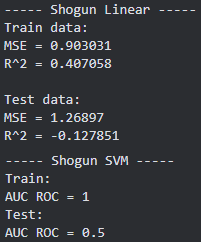
\includegraphics[width=\linewidth]{Rozdzial7/shogun}
		\caption{Wynik działania programu dla biblioteki Shogun}
		\label{fig:shogun_linear_svm}		
	\end{minipage}%
    \hspace{0.02\textwidth}
	\begin{minipage}{0.32\textwidth}
		\centering
		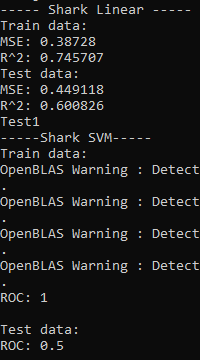
\includegraphics[width=0.7\linewidth]{Rozdzial7/shark}
		\caption{Wynik działania programu dla biblioteki Shark}
		\label{fig:shark_linear_svm}		
	\end{minipage}
\end{figure}

DOPISAĆ DALEJ !!!!!

\begin{figure}[!ht]
	
\end{figure}


\section{Wymagany nakład pracy i jakość źródeł}

W procesie pracy z poszczególnymi bibliotekami zauważono, że najmniejszą ilością potrzebnego wkładu pracy charakteryzowała się biblioteka Shark-ML. Wynika to z bardzo przyjaznej dla użytkownika składni, oraz dokładnej dokumentacji dostępnej na stronie internetowej projektu, wraz z przykładami wykorzystania poszczególnych metod. Biblioteka także bez jakichkolwiek problemów została zbudowana i zainstalowana na systemie operacyjnym Ubuntu 22.04 w środowisku WSL, pozwalając bardzo szybko przejść do docelowej pracy.

Drugą biblioteką pod względem koniecznego wkładu czasu okazał się zestaw narzędziowy Dlib. Posiada on stronę projektu z wylistowanymi klasami oraz funkcjami dostępnymi w bibliotece, jednak opis działania poszczególnych metod jest bardzo pobieżny, oraz brakuje dostępnych przykładów. Składnia biblioteki może stanowić wyzwanie dla użytkownika, gdyż nie zawsze jest oczywista, i momentami utrudnia analizę realizowanych przez program operacji.

Jako najbardziej wymagającą bibliotekę uznano Shogun. W chwili pisania niniejszej pracy, zarówno oficjalne repozytorium projektu jak i repozytorium dystrybucji dla systemu operacyjnego Ubuntu okazało się być niekompletne. Uniemożliwiło to zainstalowanie biblioteki za pomocą wbudowanego managera pakietów oraz zbudowanie jej ze względu na nienaprawione zależności do przeniesionych repozytoriów stron trzecich. Mimo przyjaźniejszej składni niż w przypadku Dlib, wspomniany wcześniej mankament sprawia, że w celu pobrania biblioteki konieczne okazało się zainstalowanie specjalnego managera pakietów \textit{nix} posiadającego starszą wersję projektu Shogun dostępną na swoim repozytorium. Z racji braku dostępnej online dokumentacji projektu Shogun oraz faktu, że generowane przykłady nie odnoszą się do API biblioteki lecz używają jej w kompletnie odrębny, nienaturalny dla projektu sposób, ustalenie funkcjonalności oraz sposobu realizacji poszczególnych zadań uczenia maszynowego musiało zostać oparte praktycznie wyłącznie o materiały dostępne w formie książkowej. Znacznie utrudnia i wydłuża to proces zastosowania biblioteki do jakiegokolwiek projektu.
\chapter{Podsumowanie}

\section{Nakład pracy}
\section{Funkcjonalności}
\section{Dostępność źródeł wiedzy i dokumentacja}


%========================================================================================
% Dodatki
%========================================================================================
\begin{appendix}
\appendix
	%\chapter{Cel dodatków w pracy}
%=================================================================================================

Do materiałów, które mogą uzupełnić pracę, oprócz rysunków, tablic, ilustracji itp. należą także dodatki, nazwane również aneksami. Dają one możliwość albo dołączenia do tekstu głównego różnorodnego rodzaju informacji dodatkowych, albo wyłączenia z tekstu głównego tych wiadomości, które nie są w nim konieczne. Niekiedy pewne wiadomości wplecione w tekst niepotrzebnie go obciążają, przerywają zasadniczy wątek lub są nadmiernie szczegółowe. Jeśli mimo to wiadomości te są użyteczne i mogą być przydatne, warto oczyścić z nich tekst główny i zgrupować je na końcu pracy w postaci dodatków.


Przykładem użycia dodatków może być opis zawartości płyty CD lub DVD dołączonej do pracy lub instrukcje laboratoryjne stworzone w oparciu o napisaną pracę.

%=================================================================================================

	%\chapter{Składanie wzorów}

W tej części nie opisywano już samych zasad tworzenia dokumentu, a zamiast tego skupiono się na przedstawieniu kilku przykładowo złożonych wzorów. W źródłach szablonu możliwe jest sprawdzenie jak wzór był pisany z wykorzystaniem notacji \LaTeX\ oraz pakietu \AmS. Więcej szczegółów zawiera rozdział ósmy świetnego opracowania oraz dokumentacja pakietu.
\begin{itemize}
\item Wzór dzielony i wyrównywany do znaku
\begin{equation}
	\begin{split}
		(a+b)^4  &= (a+b)^2 (a+b)^2 \\
					&= (a^2+2ab+b^2)(a^2+2ab+b^2) \\
					&= a^4+4a^3b+6a^2b^2+4ab^3+b^4. \\
	\end{split}
\end{equation}

\item Wzór w kilku liniach
\begin{multline}
	a+b+c+d+e+f+g+h+i+j+k+l+m+n\\
							o-p-r-s-t-u-w-x-y-z.
\end{multline}

\item Grupa wzorów
\begin{gather}
	a_1=b_1+c_1,\\
	a_2=b_2+c_2-d_2+e_2.
\end{gather}
\item Wzory z wyrównywaniem do znaku i osobną numeracją
\begin{align}
	x^2+y^2	&= 1, 					& x^3+y^3	&=1, \\
				x&=\sqrt{1-y^2},	& x 			&= \sqrt[3]{1-y^3}.
\end{align}

\begin{align}
	a_{11}& =b_{11},&
	a_{12}& =b_{12},\\
	a_{21}& =b_{21},&
	a_{22}& =b_{22}+c_{22}.
\end{align}
\item Wzory z wyrównywaniem do znaku oraz zewnętrznych marginesów i osobną numeracją 
\begin{flalign}
	a_{11}&	=b_{11},&
	a_{12}&	=b_{12},\\
	a_{21}&	=b_{21},&
	a_{22}&	=b_{22}+c_{22}.
\end{flalign}

\item Klamra
\begin{equation}
P_{r-j}=\begin{cases}
	0							& \text{jeśli $r-j$ jest nieparzyste},\\
	r!\,(-1)^{(r-j)/2}	& \text{w przeciwnym razie}.
\end{cases}
\end{equation}

\item Macierze
\begin{equation}
A=
	\begin{bmatrix}
		a	&	b	&	c		&	d	\\
		b	&	a	&	c+d	&	c-d	\\
		0	&	0	&	a+b	&	a-b	\\
		0	&	0	&	ab		&	cd	\\
	\end{bmatrix},
\end{equation}

\begin{equation}I_4=
	\begin{pmatrix}
			1 & 0 & 0 & 0 \\
		 	0 & 1 & 0 & 0 \\
			0 & 0 & 1 & 0 \\
			0 & 0 & 0 & 1 \\ 
	\end{pmatrix}
,\quad
\det{I_4}=
	\begin{vmatrix}
			1 & 0 & 0 & 0 \\
		 	0 & 1 & 0 & 0 \\
			0 & 0 & 1 & 0 \\
			0 & 0 & 0 & 1 \\ 
	\end{vmatrix}.
\end{equation}

\item Granica
\begin{equation}
\lim_{x\to 0}(1+x)^{\frac{1}{x}}=\mathrm{e}.
\end{equation}
\item Całka
\begin{equation}
\int_{0}^{1}3x^2\,\mathrm{d}x.
\end{equation}
\item Wzór z funkcjami trygonometrycznymi
\begin{equation}
\sin (\alpha \pm \beta) = \sin (\alpha) \cdot \cos (\beta) \pm \cos (\alpha) \cdot \sin (\beta).
\end{equation} 

\item Wzór Taylora
\begin{equation}
	\begin{split}f(x) &= f(a) + \frac{x-a}{1!} f^{(1)}(a) + \frac{(x-a)^2}{2!} f^{(2)}(a) + \ldots \\
							&+ \frac{(x-a)^n}{n!} f^{(n)}(a) + R_n(x,a)\\
							&= \sum\limits_{k=0}^n \left( \frac{(x-a)^k}{k!} f^{(k)}(a) \right) + R_n(x,a).
	\end{split}
\end{equation}
\end{itemize}

\end{appendix}

%========================================================================================
% Literatura
%========================================================================================

\begin{flushleft}
	\printbibliography[title={Bibliografia}]
\end{flushleft}

\end{document}
%========================================================================================
% Koniec dokumentu
%========================================================================================
